\documentclass[./main.tex]{subfiles} 
\begin{document}

\subsection{Adaptive Noise Cancellation}


\subsubsection{The Effects of Correlation on the Adaptive Line Enhancement Filter} \label{sec:3_3_a}


\subsubsection{Parameters of the Adaptive Line Enhancement Filter}
Having implemented the ALE filter, we can test two of the parameters which determine its performance: the time delay, $ \bigtriangleup $, applied in the input signal which is fed in to the Linear Predictor, and the order of the LMS filter (the heart of the Linear Predictor) itself.

The signal $S(n)$ is composed of a sine wave and noise, such that $ s(n) = x(n) + \eta(n) $ where $x(n)$ refers to the sine wave (with angular frequency $ \omega_0 = 0.01\pi$) and $ \eta(n) = v(n) + 0.5v(n-2) $ where $v(n) \sim \mathcal{N}(0,1) $.

Figure \ref{fig:3_3_b_sweeps} shows the two parameters which have been varied. In order to ensure reliable results, a `Monte Carlo' style simulation was conducted, taking the average results across ten iterations of the data. The data remained constant between the parameter sweeps, in order to ensure a fair test. Whilst there were specific parameters within which to test the time delay $ \bigtriangleup $ and filter order. But since the code was written, it was decided to explore those parameter values around and between the ones specified. The ones specified are marked on the plots as red circles, with blue stars representing other parameters tested.

Figure \ref{fig:3_3_b_delay} shows how the MSPE changes as the time delay  $ \bigtriangleup $ to the filter input $ \mathbf{u}(n) $ changes. We can see the lowest MSPE lies around $ \bigtriangleup = 4 $ and $ \bigtriangleup = 6$. Unsurprisingly, $ \bigtriangleup $ at low values shows very poor performance - since the noise in $ s(n) $ will still be correlated with $ \mathbf{u}(n) $ (as analysed in Section \ref{sec:3_3_a} ). At larger values, the MSPE also appears to get worse. By observing the output of the system, you notice that as the delay increases, the output becomes less and less in phase with the input, thus becoming less accurate not because of noise itself, but because it is out of phase with the original signal.

Figure \ref{fig:3_3_b_order} shows the relationship between the MSPE and filter order, $M$. We can see the minima of the MSPE is when $M = 5$. The Complexity of an LMS filter is $ 2M + 1 $ \cite{Dhiman2013}. Thus for every order we add to the filter, we are increasing the computational complexity of the problem. It is clear that a filter order of $M = 1$ or $M=2$ has very poor performance, but an order of 3 or 4 may be an acceptable trade off for filter order, considering the extra computational cost. This importance of additional computational cost does depend on the device and situation though - here using desktop computers, extra parameters within the bounds of the coursework cause no discernible problem in computation time. If this were for example, on an embedded low power DSP chip, this trade off may become more apparent and need to be anaylsed in further depth. In comparison to many algorithms which are proportional to $ N^2 $ (where $N$ reflects the size of the computational problem), a linear relationship is still fairly good. Thus we can be comfortable selecting the optimal order filter, 5, knowing there is little overhead in doing so.

\begin{figure}[h]
	\centering
	\begin{subfigure}[b]{0.49\textwidth}
		\resizebox{\textwidth}{2in}{% This file was created by matlab2tikz v0.4.7 (commit 84da6da3eee1f984abca8102d577f21df97f7554) running on MATLAB 8.3.
% Copyright (c) 2008--2014, Nico Schlömer <nico.schloemer@gmail.com>
% All rights reserved.
% Minimal pgfplots version: 1.3
% 
% The latest updates can be retrieved from
%   http://www.mathworks.com/matlabcentral/fileexchange/22022-matlab2tikz
% where you can also make suggestions and rate matlab2tikz.
% 
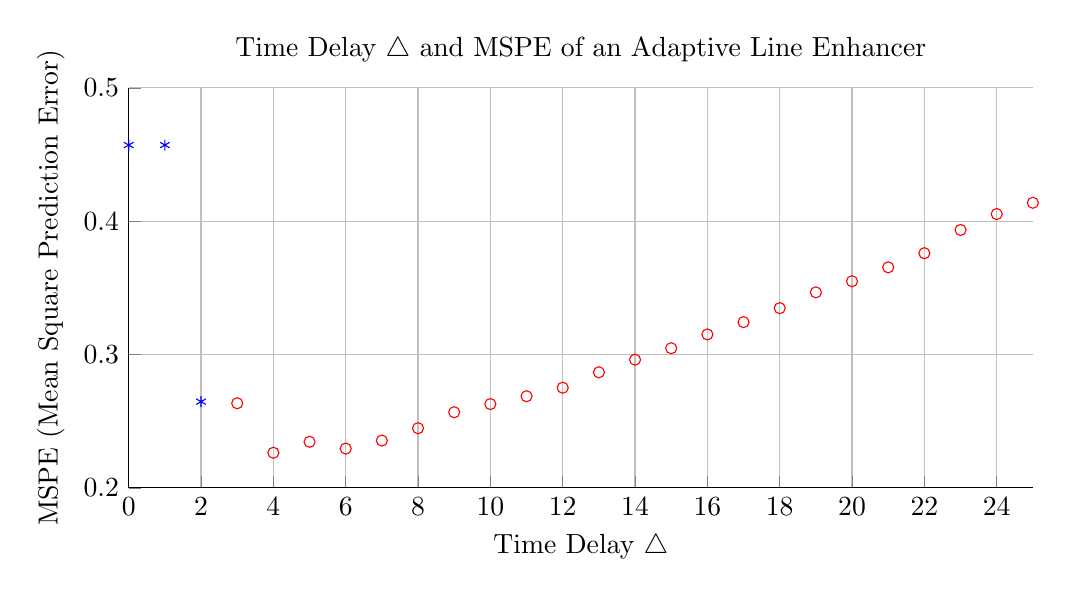
\begin{tikzpicture}

\begin{axis}[%
width=4.52083333333333in,
height=2in,
scale only axis,
xmin=0,
xmax=25,
xlabel={Time Delay $ \bigtriangleup $},
xmajorgrids,
ymin=0.2,
ymax=0.5,
ylabel={MSPE (Mean Square Prediction Error)},
ymajorgrids,
title={Time Delay $ \bigtriangleup $ and MSPE of an Adaptive Line Enhancer},
axis x line*=bottom,
axis y line*=left
]
\addplot [color=blue,only marks,mark=asterisk,mark options={solid},forget plot]
  table[row sep=crcr]{0	0.457112758906601\\
};
\addplot [color=blue,only marks,mark=asterisk,mark options={solid},forget plot]
  table[row sep=crcr]{1	0.457105598994501\\
};
\addplot [color=blue,only marks,mark=asterisk,mark options={solid},forget plot]
  table[row sep=crcr]{2	0.264648005573513\\
};
\addplot [color=red,only marks,mark=o,mark options={solid},forget plot]
  table[row sep=crcr]{3	0.263460490384655\\
};
\addplot [color=red,only marks,mark=o,mark options={solid},forget plot]
  table[row sep=crcr]{4	0.226349687179327\\
};
\addplot [color=red,only marks,mark=o,mark options={solid},forget plot]
  table[row sep=crcr]{5	0.234569847762656\\
};
\addplot [color=red,only marks,mark=o,mark options={solid},forget plot]
  table[row sep=crcr]{6	0.229458162435836\\
};
\addplot [color=red,only marks,mark=o,mark options={solid},forget plot]
  table[row sep=crcr]{7	0.235476978572889\\
};
\addplot [color=red,only marks,mark=o,mark options={solid},forget plot]
  table[row sep=crcr]{8	0.244740113347285\\
};
\addplot [color=red,only marks,mark=o,mark options={solid},forget plot]
  table[row sep=crcr]{9	0.256717932440133\\
};
\addplot [color=red,only marks,mark=o,mark options={solid},forget plot]
  table[row sep=crcr]{10	0.262847321334085\\
};
\addplot [color=red,only marks,mark=o,mark options={solid},forget plot]
  table[row sep=crcr]{11	0.268732331957349\\
};
\addplot [color=red,only marks,mark=o,mark options={solid},forget plot]
  table[row sep=crcr]{12	0.275114396677354\\
};
\addplot [color=red,only marks,mark=o,mark options={solid},forget plot]
  table[row sep=crcr]{13	0.28667927857361\\
};
\addplot [color=red,only marks,mark=o,mark options={solid},forget plot]
  table[row sep=crcr]{14	0.296155243031606\\
};
\addplot [color=red,only marks,mark=o,mark options={solid},forget plot]
  table[row sep=crcr]{15	0.304730148097582\\
};
\addplot [color=red,only marks,mark=o,mark options={solid},forget plot]
  table[row sep=crcr]{16	0.315095062870094\\
};
\addplot [color=red,only marks,mark=o,mark options={solid},forget plot]
  table[row sep=crcr]{17	0.324312346853434\\
};
\addplot [color=red,only marks,mark=o,mark options={solid},forget plot]
  table[row sep=crcr]{18	0.334793987827317\\
};
\addplot [color=red,only marks,mark=o,mark options={solid},forget plot]
  table[row sep=crcr]{19	0.346640873844623\\
};
\addplot [color=red,only marks,mark=o,mark options={solid},forget plot]
  table[row sep=crcr]{20	0.355001454398426\\
};
\addplot [color=red,only marks,mark=o,mark options={solid},forget plot]
  table[row sep=crcr]{21	0.365391974658412\\
};
\addplot [color=red,only marks,mark=o,mark options={solid},forget plot]
  table[row sep=crcr]{22	0.376014463963637\\
};
\addplot [color=red,only marks,mark=o,mark options={solid},forget plot]
  table[row sep=crcr]{23	0.393427558802103\\
};
\addplot [color=red,only marks,mark=o,mark options={solid},forget plot]
  table[row sep=crcr]{24	0.405385769010224\\
};
\addplot [color=red,only marks,mark=o,mark options={solid},forget plot]
  table[row sep=crcr]{25	0.413840200854496\\
};
\end{axis}
\end{tikzpicture}%}
		\caption{\textit{Differing delays plotted against their MSPEs}}
		\label{fig:3_3_b_delay}
	\end{subfigure}
	~ %add desired spacing between images, e. g. ~, \quad, \qquad, \hfill etc.
	%(or a blank line to force the subfigure onto a new line)
	\begin{subfigure}[b]{0.49\textwidth}
		\resizebox{\textwidth}{2in}{% This file was created by matlab2tikz v0.4.7 (commit d4c8764c3916fd1d124533205db34e93e01e5518) running on MATLAB 8.3.
% Copyright (c) 2008--2014, Nico Schlömer <nico.schloemer@gmail.com>
% All rights reserved.
% Minimal pgfplots version: 1.3
% 
% The latest updates can be retrieved from
%   http://www.mathworks.com/matlabcentral/fileexchange/22022-matlab2tikz
% where you can also make suggestions and rate matlab2tikz.
% 
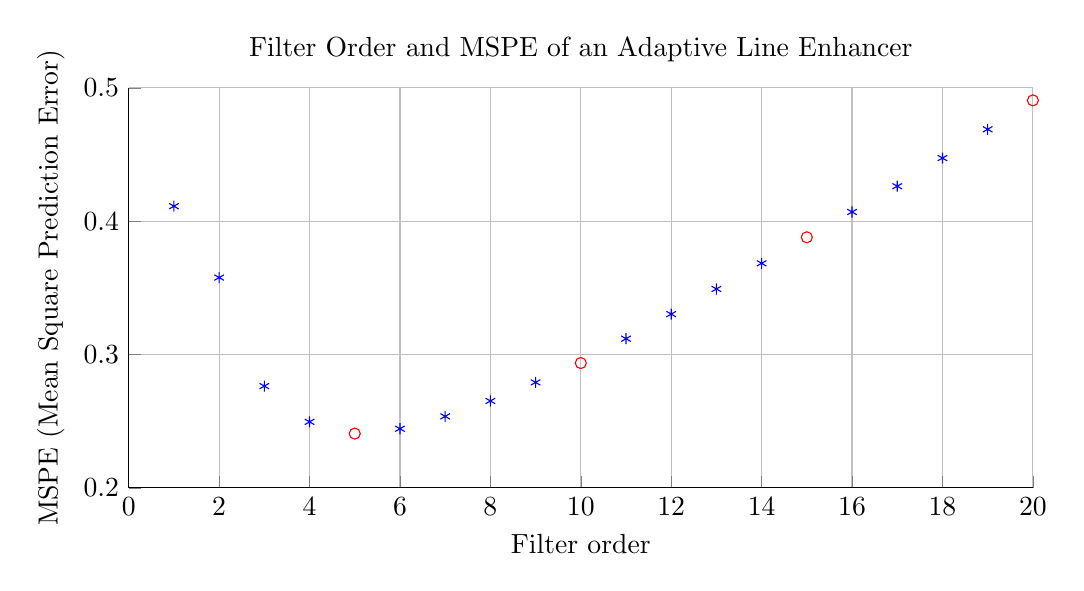
\begin{tikzpicture}

\begin{axis}[%
width=4.52083333333333in,
height=2in,
scale only axis,
xmin=0,
xmax=20,
xlabel={Filter order},
xmajorgrids,
ymin=0.2,
ymax=0.5,
ylabel={MSPE (Mean Square Prediction Error)},
ymajorgrids,
title={Filter Order and MSPE of an Adaptive Line Enhancer},
axis x line*=bottom,
axis y line*=left
]
\addplot [color=blue,only marks,mark=asterisk,mark options={solid},forget plot]
  table[row sep=crcr]{1	0.411259699209019\\
};
\addplot [color=blue,only marks,mark=asterisk,mark options={solid},forget plot]
  table[row sep=crcr]{2	0.357717205568794\\
};
\addplot [color=blue,only marks,mark=asterisk,mark options={solid},forget plot]
  table[row sep=crcr]{3	0.276328738399026\\
};
\addplot [color=blue,only marks,mark=asterisk,mark options={solid},forget plot]
  table[row sep=crcr]{4	0.249515197407873\\
};
\addplot [color=red,only marks,mark=o,mark options={solid},forget plot]
  table[row sep=crcr]{5	0.240699799461666\\
};
\addplot [color=blue,only marks,mark=asterisk,mark options={solid},forget plot]
  table[row sep=crcr]{6	0.244347593372698\\
};
\addplot [color=blue,only marks,mark=asterisk,mark options={solid},forget plot]
  table[row sep=crcr]{7	0.25362703946698\\
};
\addplot [color=blue,only marks,mark=asterisk,mark options={solid},forget plot]
  table[row sep=crcr]{8	0.265167691260922\\
};
\addplot [color=blue,only marks,mark=asterisk,mark options={solid},forget plot]
  table[row sep=crcr]{9	0.279110030587578\\
};
\addplot [color=red,only marks,mark=o,mark options={solid},forget plot]
  table[row sep=crcr]{10	0.293620204138095\\
};
\addplot [color=blue,only marks,mark=asterisk,mark options={solid},forget plot]
  table[row sep=crcr]{11	0.311873759443725\\
};
\addplot [color=blue,only marks,mark=asterisk,mark options={solid},forget plot]
  table[row sep=crcr]{12	0.330324907652155\\
};
\addplot [color=blue,only marks,mark=asterisk,mark options={solid},forget plot]
  table[row sep=crcr]{13	0.349170498512911\\
};
\addplot [color=blue,only marks,mark=asterisk,mark options={solid},forget plot]
  table[row sep=crcr]{14	0.368428472022401\\
};
\addplot [color=red,only marks,mark=o,mark options={solid},forget plot]
  table[row sep=crcr]{15	0.387931776676648\\
};
\addplot [color=blue,only marks,mark=asterisk,mark options={solid},forget plot]
  table[row sep=crcr]{16	0.406918825214346\\
};
\addplot [color=blue,only marks,mark=asterisk,mark options={solid},forget plot]
  table[row sep=crcr]{17	0.426246105232244\\
};
\addplot [color=blue,only marks,mark=asterisk,mark options={solid},forget plot]
  table[row sep=crcr]{18	0.447334585723385\\
};
\addplot [color=blue,only marks,mark=asterisk,mark options={solid},forget plot]
  table[row sep=crcr]{19	0.468931620783603\\
};
\addplot [color=red,only marks,mark=o,mark options={solid},forget plot]
  table[row sep=crcr]{20	0.490630165046867\\
};
\end{axis}
\end{tikzpicture}%}
		\caption{\textit{Differing filter orders plotted against their MSPEs}}
		\label{fig:3_3_b_order}
	\end{subfigure}
	
	\label{fig:3_3_b_sweeps}
	\caption{\textit{MSPE of the Adaptive Line Enhancer, with varying parameters of input delay and filter order}}
\end{figure}

Using the parameters $ \bigtriangleup = 4$ and $ M = 5$, we can produce a plot of the input signal without noise $x(n)$, once noise has been added, $s(n)$ and the new estimated output. As with other experiments, multiple iterations have been taken, and the mean sampled from these (as has been done in other parts of the coursework, as well). This is shown in figure \ref{fig:3_3_b_overview}. The delay on the output signal as created by $ \mathbf{u}(n) $ is apparent. We also observe that the amplitude of noise is noticeably smaller on the output than the input - so we know the ALE has had some effect to improve the signal.

\begin{figure}[h]
\centering 
\resizebox{\textwidth}{!}{% This file was created by matlab2tikz v0.4.7 (commit 84da6da3eee1f984abca8102d577f21df97f7554) running on MATLAB 8.3.
% Copyright (c) 2008--2014, Nico Schlömer <nico.schloemer@gmail.com>
% All rights reserved.
% Minimal pgfplots version: 1.3
% 
% The latest updates can be retrieved from
%   http://www.mathworks.com/matlabcentral/fileexchange/22022-matlab2tikz
% where you can also make suggestions and rate matlab2tikz.
% 
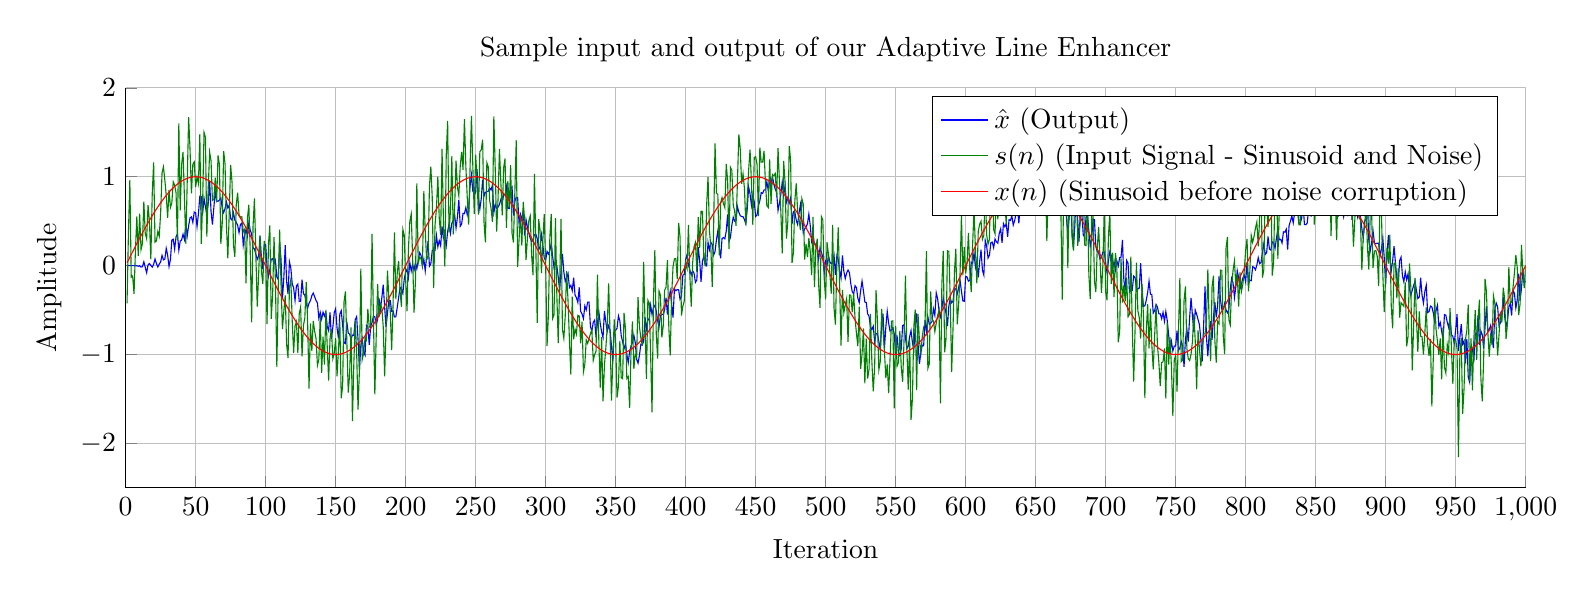
\begin{tikzpicture}

\begin{axis}[%
width=7in,
height=2in,scale only axis,
xmin=0,
xmax=1000,
xmajorgrids,
ymin=-2.5,
ymax=2,
xlabel={Iteration},
ylabel={Amplitude},
title={Sample input and output of our Adaptive Line Enhancer},
ymajorgrids,
axis x line*=bottom,
axis y line*=left,
legend style={draw=black,fill=white,legend cell align=left}
]
\addplot [color=blue,solid]
  table[row sep=crcr]{1	0\\
2	0\\
3	0\\
4	0\\
5	0\\
6	0\\
7	-0.00199102555916117\\
8	-0.000766145882907468\\
9	-0.00746507157746659\\
10	-0.0011438951318584\\
11	-0.0154885905415642\\
12	-0.0119387227500404\\
13	0.0427848745191654\\
14	-0.0192570699964584\\
15	-0.0795890699950323\\
16	0.00786769345781545\\
17	0.023256496239273\\
18	0.00258770401880402\\
19	-0.0161217301894514\\
20	0.0154240542528933\\
21	0.0741767899204495\\
22	0.0236578723521825\\
23	-0.0153577235663237\\
24	0.0181589102523915\\
25	0.0413544212909036\\
26	0.115308703485641\\
27	0.0647687153948198\\
28	0.0729800249888457\\
29	0.195631404085482\\
30	0.117527393203315\\
31	-0.0103303636097468\\
32	0.0691283937488014\\
33	0.288246744648575\\
34	0.297678253085652\\
35	0.184725620560943\\
36	0.325505429586181\\
37	0.356276183475806\\
38	0.174108371107518\\
39	0.275258756547219\\
40	0.289827651655907\\
41	0.353072460012318\\
42	0.29475452498717\\
43	0.473295512471967\\
44	0.336422258235427\\
45	0.4486193953677\\
46	0.537325529056692\\
47	0.548719739965506\\
48	0.485262466239149\\
49	0.60339231994558\\
50	0.594811699833565\\
51	0.439090958786233\\
52	0.583032457746278\\
53	0.781445091654959\\
54	0.776090382478886\\
55	0.583987350694774\\
56	0.757717025627791\\
57	0.66089315219505\\
58	0.573127301537733\\
59	0.700611399555099\\
60	0.954395158720876\\
61	0.610163317233044\\
62	0.46320599184687\\
63	0.65284970255461\\
64	0.833713529045415\\
65	0.729277017005349\\
66	0.723797255958874\\
67	0.738062863355618\\
68	0.76125907018666\\
69	0.645643724799343\\
70	0.594871924451171\\
71	0.644224672652132\\
72	0.717826634272784\\
73	0.649442226389299\\
74	0.679789933621623\\
75	0.529916362507892\\
76	0.511954843911147\\
77	0.594251012830241\\
78	0.511995285313465\\
79	0.489167592018595\\
80	0.454437434589745\\
81	0.371417072000321\\
82	0.463757610003286\\
83	0.479905517769415\\
84	0.230022877165632\\
85	0.339679479425045\\
86	0.410299481245618\\
87	0.332983059686399\\
88	0.482204801938636\\
89	0.399232411611278\\
90	0.356510112323953\\
91	0.200831136936811\\
92	0.188901872802032\\
93	0.12799976008288\\
94	0.0715280421195802\\
95	0.109104165057473\\
96	0.330129532151706\\
97	0.087886638218369\\
98	-0.0402140685563188\\
99	0.233984105806403\\
100	0.238571587526379\\
101	-0.00712391575812748\\
102	-0.121725570713935\\
103	-0.0421359505776701\\
104	0.0721021284380138\\
105	0.0790808014608243\\
106	0.0228648269417988\\
107	0.0596582485182969\\
108	-0.129044773271046\\
109	-0.156246468411231\\
110	0.245533689421426\\
111	0.0729271528200256\\
112	-0.373789756691909\\
113	-0.133404140161232\\
114	0.230089680805427\\
115	-0.180522213818034\\
116	-0.320297263558827\\
117	0.043499661175\\
118	-0.0284688806199213\\
119	-0.205313909296677\\
120	-0.248806224141722\\
121	-0.392368936303206\\
122	-0.227000090127444\\
123	-0.207340854208872\\
124	-0.402654089521316\\
125	-0.40240137412925\\
126	-0.157930901252966\\
127	-0.315094696862124\\
128	-0.331815752510444\\
129	-0.430348745202688\\
130	-0.478492811124092\\
131	-0.42174434466586\\
132	-0.393857416262089\\
133	-0.337984834078626\\
134	-0.308115565830087\\
135	-0.349620542805586\\
136	-0.391258151338648\\
137	-0.419447048129861\\
138	-0.591499675658761\\
139	-0.52517807466556\\
140	-0.60264578453679\\
141	-0.523053723564664\\
142	-0.5673475877239\\
143	-0.518891705652115\\
144	-0.684367017925629\\
145	-0.73258333092744\\
146	-0.527271532031338\\
147	-0.823431720565026\\
148	-0.695293901852767\\
149	-0.528776053524467\\
150	-0.484836006505405\\
151	-0.700898330332902\\
152	-0.817334745806778\\
153	-0.544483926674373\\
154	-0.506497048568432\\
155	-0.671957810161982\\
156	-0.868199455252385\\
157	-0.87735611301354\\
158	-0.631896515854211\\
159	-0.758065894464125\\
160	-0.770219225916565\\
161	-0.829433687399374\\
162	-0.781007685022397\\
163	-0.784024982298875\\
164	-0.606901053895351\\
165	-0.574114525429896\\
166	-0.83051928679249\\
167	-1.17014313515529\\
168	-0.89853452597676\\
169	-0.821744612880942\\
170	-0.967775824123561\\
171	-1.00696999533092\\
172	-0.670198941477381\\
173	-0.681618196665026\\
174	-0.890172808220678\\
175	-0.687949231399095\\
176	-0.638809861748195\\
177	-0.568049540422856\\
178	-0.574871343901212\\
179	-0.66326702734244\\
180	-0.600427210141353\\
181	-0.368525988729571\\
182	-0.492231132401869\\
183	-0.360673872270485\\
184	-0.214366458977919\\
185	-0.469406156291556\\
186	-0.69164247852806\\
187	-0.538959479437831\\
188	-0.39488740991298\\
189	-0.39138330761625\\
190	-0.514838527599459\\
191	-0.507982922507557\\
192	-0.577053146596337\\
193	-0.575441798089245\\
194	-0.469040743077728\\
195	-0.358150217328688\\
196	-0.244461434386716\\
197	-0.264932107374394\\
198	-0.311823858157541\\
199	-0.151802870244204\\
200	-0.0751878134568607\\
201	-0.0415194429327213\\
202	-0.136293714143652\\
203	0.0315468495961406\\
204	-0.0597236087241191\\
205	0.0143942041844737\\
206	-0.0517733023346956\\
207	0.0347448877138816\\
208	-0.0339515496309887\\
209	0.0562640907506905\\
210	0.146036095288093\\
211	0.114899860178801\\
212	-0.00632079525813114\\
213	0.0724834218515131\\
214	-0.0587118197103165\\
215	0.113275748495006\\
216	0.274509719263564\\
217	-0.00649131575053957\\
218	0.020414537906754\\
219	0.169370634995857\\
220	0.178955426803328\\
221	0.173989840470099\\
222	0.339376174007709\\
223	0.211727624335497\\
224	0.280513576388861\\
225	0.224527573132391\\
226	0.441410186285325\\
227	0.305591694716159\\
228	0.316907509979059\\
229	0.22231777206933\\
230	0.384724455383279\\
231	0.468193607347647\\
232	0.363511277068078\\
233	0.477672862735045\\
234	0.508889582088084\\
235	0.573018873942862\\
236	0.422938002004728\\
237	0.544661769811037\\
238	0.740784589037536\\
239	0.442967489184726\\
240	0.468455010792239\\
241	0.588730295810935\\
242	0.585351526136105\\
243	0.653894054337933\\
244	0.570580082134261\\
245	0.628413696229843\\
246	0.888821156995639\\
247	1.02227887169124\\
248	0.835622854241739\\
249	0.844418672085988\\
250	0.820536504045253\\
251	1.08558641739313\\
252	0.764133610294103\\
253	0.636975395635685\\
254	0.751289888888468\\
255	0.967665185404839\\
256	0.782097355985514\\
257	0.825554457273151\\
258	0.830464518728401\\
259	0.838286079147512\\
260	0.874132212185337\\
261	0.85054445889643\\
262	0.908293121878117\\
263	0.597687204437049\\
264	0.687695591209216\\
265	0.645758597196062\\
266	0.65797899415303\\
267	0.687586834697373\\
268	0.74462883961226\\
269	0.711633574805476\\
270	0.799447902407673\\
271	0.798169667572516\\
272	0.885593305776175\\
273	0.645586152085587\\
274	0.64253341080377\\
275	0.870122319027895\\
276	0.887034679232992\\
277	0.563046444724339\\
278	0.725374479443217\\
279	0.767921591330992\\
280	0.765783998041802\\
281	0.479582771055795\\
282	0.575853194022398\\
283	0.512613713766684\\
284	0.622634111005594\\
285	0.338158102994802\\
286	0.517402884032394\\
287	0.432870571507242\\
288	0.368588142130721\\
289	0.308058032368157\\
290	0.268595795433584\\
291	0.287284057193325\\
292	0.351812497392528\\
293	0.35319690312359\\
294	0.30418837760709\\
295	0.17804981473016\\
296	0.215541089566079\\
297	0.35094644048072\\
298	0.234113704657299\\
299	0.085657463474028\\
300	0.0587583329129236\\
301	0.15954613178189\\
302	0.129425347105563\\
303	0.170670212273769\\
304	0.250105487610964\\
305	0.10366172460957\\
306	-0.0254185642499514\\
307	0.0141130290749601\\
308	-0.00172781161391359\\
309	-0.128926989557269\\
310	-0.280796981383286\\
311	-0.059837710702124\\
312	0.130887440007101\\
313	-0.0718456079849847\\
314	-0.177939180036077\\
315	-0.13463759374473\\
316	-0.0876203928253484\\
317	-0.246604559268779\\
318	-0.221666694150721\\
319	-0.2808068543461\\
320	-0.135089152569774\\
321	-0.330653329103797\\
322	-0.361281212682688\\
323	-0.413939760998332\\
324	-0.243496751806242\\
325	-0.513976667378442\\
326	-0.543446225119378\\
327	-0.596138854013329\\
328	-0.452917981459305\\
329	-0.49813461586275\\
330	-0.411727853901771\\
331	-0.410036985301103\\
332	-0.684412769978712\\
333	-0.738640774960936\\
334	-0.637282193575891\\
335	-0.612647826160882\\
336	-0.805358379523656\\
337	-0.647225767121241\\
338	-0.517555392873169\\
339	-0.650125097911366\\
340	-0.746173258091948\\
341	-0.808747166942455\\
342	-0.509921288260603\\
343	-0.634078091390086\\
344	-0.738214631197746\\
345	-0.674574072493591\\
346	-0.723973478503672\\
347	-0.897834620627897\\
348	-1.07475112352434\\
349	-0.735793730385978\\
350	-0.727017554290359\\
351	-0.704483209668839\\
352	-0.564623841168548\\
353	-0.619457209368478\\
354	-0.788602483239912\\
355	-0.857444858944427\\
356	-0.93527955363334\\
357	-0.877695610428705\\
358	-0.996771907238217\\
359	-1.09218954295941\\
360	-0.966170499869425\\
361	-0.905083602996474\\
362	-0.866854969317629\\
363	-0.782337562982962\\
364	-0.864610060478855\\
365	-1.0550596266113\\
366	-1.09685479340009\\
367	-1.00867862120585\\
368	-0.884690270358512\\
369	-0.893433986426244\\
370	-0.850468062677266\\
371	-0.578889571122568\\
372	-0.70963382294108\\
373	-0.613396515458933\\
374	-0.594591822199573\\
375	-0.444270736032323\\
376	-0.550983717223735\\
377	-0.471495467178712\\
378	-0.447166779813082\\
379	-0.507903203582954\\
380	-0.618406938910878\\
381	-0.68938740858919\\
382	-0.561346141770375\\
383	-0.549512326984542\\
384	-0.546664052368475\\
385	-0.496709176143666\\
386	-0.359030495749815\\
387	-0.549426472808549\\
388	-0.375184858493267\\
389	-0.28716501836068\\
390	-0.435932828061277\\
391	-0.583101044627079\\
392	-0.259108891009325\\
393	-0.282295564486655\\
394	-0.269460325890878\\
395	-0.271761154086517\\
396	-0.379099838380413\\
397	-0.34512737424831\\
398	-0.107976868689703\\
399	-0.0968680969950371\\
400	0.0656680784270037\\
401	0.123378954527845\\
402	0.0066477359265674\\
403	-0.0500642051548049\\
404	-0.104988769160406\\
405	-0.056504104734372\\
406	-0.0855147904170734\\
407	-0.187912192138168\\
408	-0.16070822285105\\
409	0.207202006925674\\
410	0.0601361937648822\\
411	-0.182806209289777\\
412	0.0511405354349759\\
413	0.106486818116199\\
414	0.0165692864928624\\
415	-0.00133571325263244\\
416	0.260565648724987\\
417	0.179253617500881\\
418	0.263063897317437\\
419	0.236817552819522\\
420	0.119180164589013\\
421	0.158450770801204\\
422	0.292500752299489\\
423	0.389546710943932\\
424	0.207821817272297\\
425	0.0834275197642773\\
426	0.305623477211353\\
427	0.315555011813986\\
428	0.302196355405004\\
429	0.387762319209013\\
430	0.577463971192993\\
431	0.275153633463174\\
432	0.317149445327249\\
433	0.457117378313831\\
434	0.544429409251146\\
435	0.502369261277569\\
436	0.512635033470477\\
437	0.663687018294557\\
438	0.601577280647234\\
439	0.562515986095\\
440	0.551860570022385\\
441	0.55119211540348\\
442	0.517920545010311\\
443	0.46845380385669\\
444	0.640555398168316\\
445	0.886396023210865\\
446	0.80776206985098\\
447	0.677436501254152\\
448	0.789446001010086\\
449	0.71867989255955\\
450	0.552688622517635\\
451	0.568721454367775\\
452	0.677177739523173\\
453	0.729665015868632\\
454	0.82209401366659\\
455	0.812872868008719\\
456	0.852254398343493\\
457	0.851572471976841\\
458	0.944339148754235\\
459	0.846067567227073\\
460	0.961314472850341\\
461	0.914460146699515\\
462	1.00574951556814\\
463	0.915990540870483\\
464	0.860553592516989\\
465	0.823867524102249\\
466	0.620745378240824\\
467	0.701894587878513\\
468	0.802710082468311\\
469	0.938781464701199\\
470	0.787550551782153\\
471	0.897724919384353\\
472	0.712930415935413\\
473	0.764675375572766\\
474	0.703476705635358\\
475	0.76434300801301\\
476	0.468482341561279\\
477	0.609409290257679\\
478	0.602018348412824\\
479	0.510962781242846\\
480	0.463623716548092\\
481	0.592780977338654\\
482	0.688936625655779\\
483	0.518316810667209\\
484	0.370126810582715\\
485	0.411927431985336\\
486	0.438219886221085\\
487	0.469811088415032\\
488	0.5806449094928\\
489	0.451558254738308\\
490	0.274094650115529\\
491	0.338033704744004\\
492	0.244320284728647\\
493	0.244105508315932\\
494	0.176438554731368\\
495	0.0711692884294946\\
496	0.201595771288908\\
497	0.149194329739061\\
498	0.0930153847110273\\
499	-0.0904581561665942\\
500	0.0462473409814707\\
501	0.00243231409182619\\
502	0.114399428828972\\
503	0.0421427061319619\\
504	0.019999799728057\\
505	0.0393500868926022\\
506	0.116778291288801\\
507	-0.102703278034316\\
508	0.108191283320782\\
509	0.0711463471184554\\
510	-0.0583927911514153\\
511	-0.138411665140961\\
512	0.114723948234123\\
513	-0.0636077199611603\\
514	-0.144806198236795\\
515	-0.082302830751844\\
516	-0.0491618935989711\\
517	-0.0785773038962827\\
518	-0.206492958989052\\
519	-0.292155836962093\\
520	-0.319875873147297\\
521	-0.226072428408524\\
522	-0.246163421450734\\
523	-0.36559736780492\\
524	-0.415974776356222\\
525	-0.280479210121231\\
526	-0.174060315075046\\
527	-0.283610445731984\\
528	-0.408521118754063\\
529	-0.415559205265358\\
530	-0.542158623159627\\
531	-0.569549441717858\\
532	-0.686771361393827\\
533	-0.719450532136873\\
534	-0.681018841134337\\
535	-0.858430273996841\\
536	-0.76764159018292\\
537	-0.760876739723188\\
538	-0.85243717020472\\
539	-0.939225269606256\\
540	-0.68183679080709\\
541	-0.540831247224229\\
542	-0.930222363230104\\
543	-0.688617081636441\\
544	-0.514206393411139\\
545	-0.647608962214666\\
546	-0.735890660563445\\
547	-0.724503190941864\\
548	-0.698477985512945\\
549	-0.767517292937004\\
550	-0.996437817874938\\
551	-0.783510635697308\\
552	-0.978419414324571\\
553	-1.00833669069883\\
554	-0.936812524870027\\
555	-0.673253419584233\\
556	-0.665144350056322\\
557	-0.810939254803533\\
558	-0.931302614239998\\
559	-0.905789298987268\\
560	-0.798880234691247\\
561	-0.730421293142736\\
562	-0.866168926706018\\
563	-0.950598074764708\\
564	-0.67414246319161\\
565	-0.537286405849674\\
566	-0.877180670290969\\
567	-1.10564992168977\\
568	-0.98017194722291\\
569	-0.893992244369497\\
570	-0.900662866841995\\
571	-0.614009127581355\\
572	-0.736761146588911\\
573	-0.573851455303102\\
574	-0.659683419935141\\
575	-0.647154629196257\\
576	-0.628609701180642\\
577	-0.48737557023241\\
578	-0.558577548185908\\
579	-0.305171980604269\\
580	-0.372247154232022\\
581	-0.507789278519077\\
582	-0.575594296029879\\
583	-0.485771513518578\\
584	-0.360367673644097\\
585	-0.458682615801247\\
586	-0.537955411250679\\
587	-0.681102456027208\\
588	-0.454306829009057\\
589	-0.36612167462459\\
590	-0.418011187270798\\
591	-0.396979970924195\\
592	-0.252721542690874\\
593	-0.26543066708976\\
594	-0.31755101217708\\
595	-0.246164188901291\\
596	-0.165035481603622\\
597	-0.288377727332005\\
598	-0.397502200335717\\
599	-0.399867714932617\\
600	-0.120324634823389\\
601	-0.126483412351469\\
602	-0.174190015036516\\
603	-0.165114857151143\\
604	0.038374635782764\\
605	0.021633326667722\\
606	0.143960705813444\\
607	-0.0202628148832196\\
608	0.0492281207959032\\
609	-0.131538948472118\\
610	0.042957395595262\\
611	0.178631135839994\\
612	-0.0538192412685167\\
613	-0.106622260083159\\
614	0.284615090178936\\
615	0.220470049374929\\
616	0.0855829121308054\\
617	0.116404824932886\\
618	0.258395510924905\\
619	0.264732452865226\\
620	0.201171530161955\\
621	0.300970823973181\\
622	0.269208389215355\\
623	0.253348931691705\\
624	0.362702321076204\\
625	0.413415825771745\\
626	0.256798848563139\\
627	0.473676311777122\\
628	0.438173738865381\\
629	0.472448593919163\\
630	0.325365969256883\\
631	0.516992317598702\\
632	0.509205328920079\\
633	0.560367025984597\\
634	0.457196894071505\\
635	0.505456750011886\\
636	0.587429913805485\\
637	0.667763825689915\\
638	0.476137721155842\\
639	0.699533818823247\\
640	0.748007584254939\\
641	0.698359313916181\\
642	0.753361824684729\\
643	0.863297936712952\\
644	0.825521624563509\\
645	0.828572131882284\\
646	0.930326164425059\\
647	0.868999474154728\\
648	0.731012409283273\\
649	0.699841280224803\\
650	0.960713168986389\\
651	0.858781228993183\\
652	0.922925454043379\\
653	0.887276824618533\\
654	1.01403401741196\\
655	1.03900275138355\\
656	1.0464059306483\\
657	0.813140701824668\\
658	1.05604016923932\\
659	0.897655626401414\\
660	0.976934512452778\\
661	0.981431757172901\\
662	0.995440399376633\\
663	0.759587516852996\\
664	0.82091366272288\\
665	0.662986120074669\\
666	0.677590178144137\\
667	0.823458293893591\\
668	0.788473526323766\\
669	0.795244476114903\\
670	0.670389719008407\\
671	0.75612612476921\\
672	0.53409996605293\\
673	0.354427733822164\\
674	0.55514369778572\\
675	0.80651487763047\\
676	0.373256930288757\\
677	0.194916368161515\\
678	0.450986354417442\\
679	0.84643763771304\\
680	0.521070341725461\\
681	0.269980770037821\\
682	0.668203223835273\\
683	0.58591427065513\\
684	0.347236746463386\\
685	0.317420557259548\\
686	0.549029288546824\\
687	0.575336250348126\\
688	0.396212264337268\\
689	0.21669046228287\\
690	0.298816642097809\\
691	0.524037483791077\\
692	0.516954879407573\\
693	0.214289578767656\\
694	0.157482208459045\\
695	0.142253262809177\\
696	0.0773606406633782\\
697	0.0948309113603279\\
698	0.151938531829854\\
699	0.154602960996568\\
700	0.0335819464976309\\
701	-0.082511757476297\\
702	0.0518576966271238\\
703	0.159263390991608\\
704	0.116531899896819\\
705	-0.0359911212821424\\
706	0.0475066009836978\\
707	-0.0504572126284515\\
708	0.0541640322983626\\
709	-0.00299945655368837\\
710	0.0912041440823129\\
711	0.0955976196810132\\
712	0.288987152486399\\
713	-0.163085650390442\\
714	-0.276956928009826\\
715	0.0593225594172983\\
716	0.0281880318089265\\
717	-0.295293526698778\\
718	-0.279900085030065\\
719	-0.276996627411763\\
720	-0.117343049111174\\
721	-0.133876373619919\\
722	-0.248721819971272\\
723	-0.263546414983977\\
724	-0.252914408349178\\
725	0.0270754661287338\\
726	-0.289704125591452\\
727	-0.457369972378739\\
728	-0.452717513419435\\
729	-0.390067822861302\\
730	-0.303776868289222\\
731	-0.17361082717363\\
732	-0.320987727241119\\
733	-0.325659161424245\\
734	-0.533736630399667\\
735	-0.505330252711621\\
736	-0.43655444183859\\
737	-0.465290466418301\\
738	-0.542618691423572\\
739	-0.54181721725745\\
740	-0.596591204089425\\
741	-0.525668438391159\\
742	-0.625829192130081\\
743	-0.515452160578246\\
744	-0.618474015514007\\
745	-0.777813069984126\\
746	-0.959369902248443\\
747	-0.853749238202037\\
748	-0.959453515389805\\
749	-0.904444937293889\\
750	-0.905297236321374\\
751	-0.73243246932108\\
752	-0.953436057884067\\
753	-0.926631763152217\\
754	-0.853138901748263\\
755	-0.910908075309327\\
756	-1.13713887227306\\
757	-0.82430964212707\\
758	-0.71385894103636\\
759	-0.853975993909793\\
760	-0.585050198150118\\
761	-0.36173366279202\\
762	-0.562933152845267\\
763	-0.748814064434993\\
764	-0.499612205876927\\
765	-0.545688252729471\\
766	-0.606190011815717\\
767	-0.664632209085201\\
768	-0.829732521819559\\
769	-1.07575509369564\\
770	-0.662955628890862\\
771	-0.233407399490081\\
772	-0.801541498947696\\
773	-1.01958270481412\\
774	-0.746704717129217\\
775	-0.622624705962925\\
776	-0.834965989471901\\
777	-0.58115812596501\\
778	-0.407807506681795\\
779	-0.582099898802366\\
780	-0.439321958175742\\
781	-0.121321786615296\\
782	-0.382998029815396\\
783	-0.493561001062488\\
784	-0.488921460613771\\
785	-0.424737444192607\\
786	-0.498881805044086\\
787	-0.531284984777085\\
788	-0.494354877913889\\
789	-0.259940514856308\\
790	-0.141333699742312\\
791	-0.193705022751361\\
792	-0.359922170884638\\
793	-0.235301107894968\\
794	-0.0554700553007867\\
795	-0.136847536010948\\
796	-0.25957950494245\\
797	-0.209089160445904\\
798	-0.137340052282329\\
799	-0.108031950890353\\
800	-0.183571602832609\\
801	0.0345222393970454\\
802	-0.204691537245422\\
803	-0.162740405863088\\
804	-0.16891309756919\\
805	-0.0117157668425073\\
806	-0.019443602141569\\
807	-0.0469732701052909\\
808	0.00766668005361047\\
809	0.0891721022406494\\
810	0.0221289884494186\\
811	0.0360489560934018\\
812	0.150284932689253\\
813	0.246637465657177\\
814	0.125607776344707\\
815	0.145597027044416\\
816	0.327842952818542\\
817	0.185830760994969\\
818	0.176021372762237\\
819	0.266668507218223\\
820	0.254374212817331\\
821	0.194737126804811\\
822	0.309616815857374\\
823	0.407558057241483\\
824	0.290334841860807\\
825	0.296390768691957\\
826	0.254622209987569\\
827	0.380647712580395\\
828	0.37667226701872\\
829	0.410427216532974\\
830	0.179707833673789\\
831	0.447475279066467\\
832	0.501910726105839\\
833	0.557585776740438\\
834	0.48061607021884\\
835	0.602450553970872\\
836	0.813385830842534\\
837	0.630008759419513\\
838	0.475018927903791\\
839	0.473894932036867\\
840	0.534999172503444\\
841	0.696308714726114\\
842	0.462296813426216\\
843	0.460724590836661\\
844	0.480418724533285\\
845	0.63782810900014\\
846	0.568077627425784\\
847	0.560033495652515\\
848	0.623742011005992\\
849	0.732933663016339\\
850	0.88201283166078\\
851	0.771988010357052\\
852	0.655581605838023\\
853	0.657921441233799\\
854	0.70646217617484\\
855	0.76003552264541\\
856	0.618853974997347\\
857	0.778218394825194\\
858	0.857638822202932\\
859	0.697750775813767\\
860	0.846923431003603\\
861	0.738640806031863\\
862	0.618345934354791\\
863	0.698667582994944\\
864	0.779150064446034\\
865	0.672169878979035\\
866	0.549770167211897\\
867	0.768460662261341\\
868	0.635257006425918\\
869	0.635261081460224\\
870	0.549372002020791\\
871	0.642003777545501\\
872	0.627451087211883\\
873	0.571839776667211\\
874	0.628314408714937\\
875	0.778428489369243\\
876	0.51672755511032\\
877	0.63791534705764\\
878	0.780323258044938\\
879	0.618509742185429\\
880	0.546600122568475\\
881	0.720290252272727\\
882	0.550337940753062\\
883	0.41814163479945\\
884	0.307919725060038\\
885	0.499853184886134\\
886	0.520161135996128\\
887	0.714013729010765\\
888	0.273439604143174\\
889	0.167949750202472\\
890	0.261492511356607\\
891	0.391199064485752\\
892	0.253830600318006\\
893	0.247878781797958\\
894	0.251615158890257\\
895	0.25181007506588\\
896	0.106447974254638\\
897	0.191537642996201\\
898	0.308134473863821\\
899	0.0864761964741605\\
900	-0.212335870349549\\
901	0.144792311843977\\
902	0.343850153042645\\
903	0.0874436911936712\\
904	-0.0582373325893029\\
905	0.0523869911171848\\
906	0.219846924345201\\
907	0.0321155404300482\\
908	-0.14657955965604\\
909	-0.203899963961539\\
910	0.058104426519743\\
911	0.0957069903786524\\
912	-0.116395707594971\\
913	-0.182131548885477\\
914	-0.0698067808786876\\
915	-0.159217908198166\\
916	-0.0932911941499725\\
917	-0.261705243428127\\
918	-0.333441445756158\\
919	-0.276628616315482\\
920	-0.223894189729996\\
921	-0.173097896314471\\
922	-0.281223499739776\\
923	-0.36936175857865\\
924	-0.353686744093762\\
925	-0.136332332753186\\
926	-0.332415818174261\\
927	-0.421428902956695\\
928	-0.291429461154243\\
929	-0.220023869971373\\
930	-0.527707285851167\\
931	-0.517304824552557\\
932	-0.454910662834024\\
933	-0.464025213187917\\
934	-0.527426994313544\\
935	-0.629915628432878\\
936	-0.504289449497797\\
937	-0.446299450125169\\
938	-0.686613457567941\\
939	-0.640749747162455\\
940	-0.73606064590141\\
941	-0.835045253009571\\
942	-0.55102052178241\\
943	-0.556700875934844\\
944	-0.636522288560826\\
945	-0.69618817118419\\
946	-0.585258433286389\\
947	-0.776568227000704\\
948	-0.795130123880258\\
949	-0.8749490313022\\
950	-0.72538979022555\\
951	-0.546534024143478\\
952	-0.95949055854218\\
953	-0.806773839978851\\
954	-0.658447237634441\\
955	-0.882294722186273\\
956	-0.8472795136424\\
957	-1.09960758876109\\
958	-0.823554887038721\\
959	-1.25449561797781\\
960	-1.3109658107262\\
961	-0.982013912659969\\
962	-0.936841995574156\\
963	-1.08442368337181\\
964	-0.761168670696694\\
965	-0.78815276695812\\
966	-0.558505364815048\\
967	-0.891480867181614\\
968	-0.735170635027955\\
969	-0.777118541926563\\
970	-0.931898160525119\\
971	-0.696384985808778\\
972	-0.459295966989059\\
973	-0.735923096373303\\
974	-0.720970197296635\\
975	-0.672050783200447\\
976	-0.818306481338229\\
977	-0.926069512178673\\
978	-0.485227519455165\\
979	-0.421864845520357\\
980	-0.465386574008653\\
981	-0.676802914271864\\
982	-0.641088413819985\\
983	-0.570233732612348\\
984	-0.351783722520798\\
985	-0.573459652453132\\
986	-0.685172362682408\\
987	-0.621152196536119\\
988	-0.466266834201544\\
989	-0.426791733081662\\
990	-0.560337675028176\\
991	-0.277681528398188\\
992	-0.31117473232686\\
993	-0.476644912483058\\
994	-0.383852245574027\\
995	-0.0910706573695292\\
996	-0.394310054693832\\
997	-0.258071277197008\\
998	-0.0556112200482027\\
999	-0.167015569292188\\
1000	-0.188205930522682\\
};
\addlegendentry{$\hat{x} $ (Output)};

\addplot [color=black!50!green,solid]
  table[row sep=crcr]{1	-0.422987193463623\\
2	0.367665295400333\\
3	0.965701131608576\\
4	-0.129739517872119\\
5	-0.115756597763504\\
6	-0.318080634054704\\
7	0.171443172050897\\
8	0.552909786823387\\
9	0.111598328006877\\
10	0.585172478092126\\
11	0.180407773957908\\
12	0.248481598724005\\
13	0.720290543914178\\
14	0.364834339771426\\
15	0.303044839446141\\
16	0.681434667592683\\
17	0.498765983751313\\
18	0.0705187899926028\\
19	0.80599282656278\\
20	1.1605451352666\\
21	0.264509259341783\\
22	0.278839546134067\\
23	0.384842278968897\\
24	0.329234149242289\\
25	0.592380974530917\\
26	1.04266235564082\\
27	1.11150508453433\\
28	0.962973800048397\\
29	0.791665256249454\\
30	0.538802568969212\\
31	0.851516990894421\\
32	0.654901207240331\\
33	0.705727595373498\\
34	0.942881967907602\\
35	0.905711875996249\\
36	0.822377881097996\\
37	0.286515580635601\\
38	1.5995553908388\\
39	0.622101558895313\\
40	1.13976177146611\\
41	1.28017937434728\\
42	0.765444266226589\\
43	0.245896849588697\\
44	0.950337723559462\\
45	1.671230422797\\
46	1.30925977089156\\
47	0.812526499650889\\
48	1.1401484866779\\
49	1.16712254591277\\
50	0.884858138857317\\
51	0.998148714578203\\
52	0.924258007281299\\
53	1.48029214930006\\
54	0.244786350119877\\
55	0.707029148721094\\
56	1.49923840198319\\
57	1.44414769644842\\
58	0.327491801735904\\
59	0.879859929945525\\
60	1.27625363347311\\
61	1.18089698055207\\
62	0.733306237605915\\
63	0.747158753978446\\
64	0.988858358024128\\
65	0.711328950711561\\
66	1.24036725621636\\
67	1.13822969121274\\
68	0.244558955676161\\
69	0.47780309393082\\
70	1.28826189022248\\
71	1.14785671526541\\
72	0.452233252453422\\
73	0.0823629896023944\\
74	0.594617640912281\\
75	1.13373285125953\\
76	0.939265341847842\\
77	0.237809823806049\\
78	0.0987649162978081\\
79	0.683364588037961\\
80	0.822061485773898\\
81	0.570749652164912\\
82	0.545273922186052\\
83	0.550365301731108\\
84	0.380017252672683\\
85	0.409131323524026\\
86	-0.199397356701494\\
87	0.534729524181391\\
88	0.684851379326422\\
89	0.16040829036547\\
90	-0.636844677184856\\
91	0.439731734647471\\
92	0.757358667880901\\
93	0.132325345931298\\
94	-0.460528420491904\\
95	-0.104555958441868\\
96	0.339442071441078\\
97	-0.0654487223107544\\
98	-0.204792376607681\\
99	0.278542764399076\\
100	0.156866451134759\\
101	-0.656359603506427\\
102	0.233916013306119\\
103	0.453337247507035\\
104	-0.599446827753515\\
105	-0.325164935289312\\
106	0.32085592119047\\
107	-0.180753102705497\\
108	-1.13973475251768\\
109	-0.24528789715668\\
110	0.405018602047061\\
111	-0.212468306552941\\
112	-0.714445167388089\\
113	-0.514700678815686\\
114	-0.334462702386076\\
115	-0.885683032242607\\
116	-1.0388771617616\\
117	-0.246031797735541\\
118	-0.155762425041052\\
119	-0.625931120910387\\
120	-0.98309170268418\\
121	-0.678181462747527\\
122	-0.631932032784189\\
123	-0.982629058212951\\
124	-0.54190253403403\\
125	-0.464816465046983\\
126	-1.0200543260868\\
127	-0.673600582543542\\
128	-0.587457594873718\\
129	-0.186413333390882\\
130	-0.641222368030653\\
131	-1.38228795654353\\
132	-0.650843193454837\\
133	-0.958980592508669\\
134	-0.622691750618276\\
135	-0.735838198850659\\
136	-0.820760873025134\\
137	-1.12308594072249\\
138	-1.05527748392793\\
139	-0.560847875241884\\
140	-1.20694349848098\\
141	-0.799655067137348\\
142	-1.1139870593661\\
143	-0.505728902065666\\
144	-0.911592042961856\\
145	-1.29248658711922\\
146	-0.817502839006449\\
147	-0.710786842879045\\
148	-1.04590049448486\\
149	-0.984787965109705\\
150	-0.816191675931922\\
151	-1.24449307941313\\
152	-0.947624715048146\\
153	-0.629491356423615\\
154	-1.49124059522242\\
155	-1.35292903671298\\
156	-0.406378737122216\\
157	-0.291065727325327\\
158	-0.846679218226706\\
159	-1.42769613779046\\
160	-1.22041887572966\\
161	-0.695105329571839\\
162	-1.74948672406385\\
163	-1.10086560049545\\
164	-0.621566683092545\\
165	-0.970868387307866\\
166	-1.62041202223599\\
167	-1.17271771546567\\
168	-0.0325577330113289\\
169	-1.05431916448992\\
170	-0.985764069847421\\
171	-0.811061914705413\\
172	-0.837761766931487\\
173	-0.486447059116894\\
174	-0.690937599964972\\
175	-0.681159947431198\\
176	0.356918014443069\\
177	-0.598477094236455\\
178	-1.44880318254372\\
179	-0.780559303117453\\
180	-0.205968608164798\\
181	-0.57518216280791\\
182	-0.432336519772061\\
183	-0.475827235206897\\
184	-0.687673253465225\\
185	-1.24586631570584\\
186	-0.722784182898426\\
187	-0.0548465640448661\\
188	-0.360886153919092\\
189	-0.507214337280425\\
190	-0.951267198086018\\
191	-0.454918562110641\\
192	0.374673427657417\\
193	-0.377702333713476\\
194	-0.0844023782516043\\
195	0.0541815180803692\\
196	-0.282672540073668\\
197	-0.46214416980329\\
198	0.410095922433781\\
199	0.343574676925836\\
200	-0.150718654214489\\
201	-0.512752438355964\\
202	0.191807436451421\\
203	0.499057472408189\\
204	0.581742442153219\\
205	0.0851644506182658\\
206	-0.528184954558744\\
207	-0.176867478949151\\
208	0.926046798237317\\
209	0.0275170553827878\\
210	0.094359344213107\\
211	0.078914482241218\\
212	0.000227443358765944\\
213	0.83757656248131\\
214	0.391114432260964\\
215	0.0634583199544947\\
216	0.105128757242684\\
217	0.891422268125245\\
218	1.11470066255819\\
219	0.770540219687397\\
220	-0.253743591071594\\
221	0.457217241687263\\
222	0.641891653545567\\
223	1.00125479640247\\
224	0.535886776799386\\
225	0.343597854812924\\
226	1.31278520995357\\
227	0.504941404850964\\
228	-0.0110721579481095\\
229	1.24380238779272\\
230	1.62737636358465\\
231	0.373908456498029\\
232	0.612032553831816\\
233	1.23202513371673\\
234	0.352219177895248\\
235	0.654371217736573\\
236	1.18128905571792\\
237	0.882283756780199\\
238	0.786977263109819\\
239	1.1195166480033\\
240	1.28049713268084\\
241	1.07897328382949\\
242	1.64728441472033\\
243	1.12274012249349\\
244	0.770280296395397\\
245	0.460530540622244\\
246	1.09587192417583\\
247	1.68406768461147\\
248	1.11471057586056\\
249	0.581551965454169\\
250	1.25002370791807\\
251	0.964270751753041\\
252	0.574524699228069\\
253	1.28314812789996\\
254	1.3027079093613\\
255	1.41741510974811\\
256	0.482600600981861\\
257	0.260970366353599\\
258	1.15892268307544\\
259	1.11097899192741\\
260	0.735764917122888\\
261	0.646783205215909\\
262	0.491909501061067\\
263	1.68050657129373\\
264	1.08960116224472\\
265	0.381918829085451\\
266	0.749039719822177\\
267	1.31325301837531\\
268	0.942742638038919\\
269	0.5648257250357\\
270	1.10201706695254\\
271	1.20470209346062\\
272	0.424139059896112\\
273	0.954299129461713\\
274	0.653077600174873\\
275	1.13016220311473\\
276	0.364113093077624\\
277	0.260847132778792\\
278	0.822699105570053\\
279	1.41061487306346\\
280	-0.0158073493344993\\
281	0.291260884120374\\
282	0.56545982385851\\
283	0.226470593699498\\
284	0.716266287525312\\
285	0.51515036084367\\
286	0.0621646628775423\\
287	0.315899813725501\\
288	0.506414297768084\\
289	0.560490295863633\\
290	0.110881652275303\\
291	-0.105575293124634\\
292	1.03138466352317\\
293	0.202293350694399\\
294	-0.644228982178872\\
295	0.5237436431879\\
296	0.401647783760928\\
297	-0.0836468250937588\\
298	0.28333857038048\\
299	0.580376404057932\\
300	0.0176222645605248\\
301	-0.905197231232141\\
302	-0.542899805521241\\
303	0.317562556000453\\
304	0.582671843824776\\
305	-0.594596845154827\\
306	-0.5525878097614\\
307	0.533506214762894\\
308	-0.333808062556189\\
309	-0.871574583663542\\
310	-0.219165378472774\\
311	0.526859431873668\\
312	-0.720259199642806\\
313	-0.817000482089351\\
314	-0.564800291100633\\
315	-0.0592536736875871\\
316	-0.39807586115059\\
317	-0.84026953560238\\
318	-1.22523203887198\\
319	-0.349180743470394\\
320	-0.828873754554672\\
321	-0.715691179081332\\
322	-0.76989012870525\\
323	-0.55869547442376\\
324	-0.567452677291994\\
325	-0.874824100664833\\
326	-0.630739134768349\\
327	-1.19437794895013\\
328	-1.11027314350612\\
329	-0.835797127049469\\
330	-0.874046051931089\\
331	-0.820958609088283\\
332	-0.765816840836664\\
333	-0.722239441526881\\
334	-1.06575037573917\\
335	-0.999850533931019\\
336	-0.963489875282842\\
337	-0.100895017033699\\
338	-0.852112730604495\\
339	-1.37117574754122\\
340	-0.804177505893474\\
341	-1.52570867781902\\
342	-1.11891244298199\\
343	-0.926189140135569\\
344	-0.692800448483775\\
345	-0.199555921116631\\
346	-0.750665019536027\\
347	-1.51826142896509\\
348	-1.05693753890659\\
349	-0.605275468502197\\
350	-0.844787500720491\\
351	-1.4831481410115\\
352	-1.35784857473164\\
353	-0.847648825520833\\
354	-1.2611453453255\\
355	-1.27232844872087\\
356	-0.532013986212761\\
357	-0.708730679371204\\
358	-1.27199288642058\\
359	-1.2490537172577\\
360	-1.6003816948545\\
361	-0.954628523689411\\
362	-0.628073751272526\\
363	-1.16108946353151\\
364	-0.998719845063578\\
365	-1.03341052445327\\
366	-0.355049442430464\\
367	-0.687853765325653\\
368	-0.811861840894579\\
369	-0.898861692172257\\
370	0.0422351116442289\\
371	-0.660690943936108\\
372	-1.27463721066477\\
373	-0.388065658956641\\
374	-0.422213976839669\\
375	-1.01644611007265\\
376	-1.64941392744923\\
377	-0.398811906252993\\
378	0.174129674107055\\
379	-0.765377643989011\\
380	-1.04634037506855\\
381	-0.285726002474075\\
382	-0.333945839612095\\
383	-0.807630611985276\\
384	-0.678598988019651\\
385	-0.276590333720583\\
386	-0.244379844350032\\
387	0.0618593641811749\\
388	-0.702358198973739\\
389	-1.00916564564984\\
390	-0.335621600704927\\
391	-0.0113059391479387\\
392	0.0767798875113527\\
393	0.0806051049266436\\
394	-0.151199294719352\\
395	0.482052406747308\\
396	0.323286046640461\\
397	-0.561965242969575\\
398	-0.456658516644507\\
399	-0.400327949892903\\
400	0.0292058115073763\\
401	-0.0314659184346711\\
402	0.457799433701715\\
403	-0.10530572897861\\
404	-0.460534858729766\\
405	0.0300813892197391\\
406	0.213125436487608\\
407	0.261988398634925\\
408	-0.0700200987984113\\
409	0.544671400439648\\
410	0.197881530328657\\
411	0.612743789897652\\
412	0.609688293587841\\
413	0.0876506592165224\\
414	-0.00729793940029635\\
415	0.681179108609815\\
416	0.998623967583502\\
417	0.394138083693094\\
418	0.209317990761616\\
419	-0.239507411342067\\
420	0.44428113103641\\
421	1.37480851987303\\
422	0.81770651350329\\
423	0.800610883745872\\
424	0.116179430889579\\
425	0.707407443830861\\
426	0.765791795437276\\
427	0.697440732219377\\
428	0.652671741250312\\
429	1.14528805742545\\
430	0.954211006095176\\
431	0.187440263413923\\
432	1.10636754513122\\
433	1.07082954346202\\
434	0.681864394636733\\
435	0.614119699025242\\
436	0.447619919187785\\
437	0.951276056303674\\
438	1.4767173657676\\
439	1.3142565620665\\
440	0.919260733939388\\
441	1.03321514804675\\
442	0.868932401537245\\
443	0.461368386702671\\
444	0.745501181207064\\
445	1.07420129316131\\
446	1.30563804679167\\
447	0.941104284564121\\
448	0.457334335536737\\
449	1.21596547289\\
450	1.22589497432204\\
451	1.14068719595487\\
452	0.557060706752702\\
453	1.32872851268487\\
454	1.16496292995037\\
455	1.16442370791931\\
456	1.29181486389327\\
457	0.928147803079784\\
458	0.674871271803156\\
459	0.654999926420014\\
460	1.19581406751826\\
461	0.696270003081125\\
462	1.02115127154355\\
463	1.01255780815102\\
464	1.03705652243941\\
465	0.772729052811979\\
466	1.32212323560604\\
467	0.944720236938844\\
468	0.610115129268867\\
469	0.138976264819413\\
470	1.17919564686723\\
471	0.93980213294768\\
472	0.303486772090318\\
473	0.499572445239088\\
474	1.34433896520982\\
475	1.18477819721832\\
476	0.0310683324417082\\
477	0.148744823027856\\
478	0.730862584338491\\
479	0.925597649602576\\
480	0.608439788657359\\
481	0.518557129887253\\
482	0.400690411365046\\
483	0.753887676437488\\
484	0.693290152360201\\
485	0.0674743400964308\\
486	0.243449958470869\\
487	0.0971416465187568\\
488	0.308966632501396\\
489	0.159391085245626\\
490	-0.107547562117832\\
491	0.548914079491502\\
492	-0.242478408934098\\
493	0.192958607931949\\
494	0.302222923977196\\
495	-0.211564811697975\\
496	-0.474987025866641\\
497	0.550047480475885\\
498	0.51178226970498\\
499	-0.153239885805688\\
500	-0.377972238665219\\
501	0.263066758447071\\
502	0.12900270084411\\
503	-0.0881559058745484\\
504	-0.315660029094001\\
505	0.459211712317577\\
506	-0.478884908719499\\
507	-0.664416698867196\\
508	0.00766315047337562\\
509	0.431699350050612\\
510	-0.228092393639649\\
511	-0.899465548441889\\
512	-0.271993939344973\\
513	-0.530021665422971\\
514	-0.444378442545339\\
515	-0.370184956510131\\
516	-0.858652257391927\\
517	-0.329815623818951\\
518	-0.33301264094274\\
519	-0.52317266996072\\
520	-0.315098466707677\\
521	-0.593203000106071\\
522	-0.762227600734894\\
523	-0.906152683638693\\
524	-0.461107022560099\\
525	-1.16112779855328\\
526	-0.99478577513115\\
527	-0.707252565610599\\
528	-1.32328175358664\\
529	-0.822403233185372\\
530	-1.27080826858889\\
531	-1.16650496755265\\
532	-0.543268485517302\\
533	-1.07200694784394\\
534	-1.41309102496404\\
535	-1.14292214828539\\
536	-0.276980295566263\\
537	-0.624484269273959\\
538	-1.17229743466069\\
539	-1.08194625260466\\
540	-0.485379271960286\\
541	-0.725724300116361\\
542	-0.963123916828582\\
543	-1.26504076782623\\
544	-1.11176515062615\\
545	-1.43288693339307\\
546	-1.04888586449348\\
547	-0.625575487830951\\
548	-0.621273695569185\\
549	-1.6044940083112\\
550	-0.677830377783635\\
551	-1.13209599827718\\
552	-1.0886742775328\\
553	-0.734820996444306\\
554	-1.14547269924306\\
555	-1.30728679575897\\
556	-0.833825351688716\\
557	-0.110970868017548\\
558	-0.931916812654798\\
559	-1.39335538158798\\
560	-0.832743130665029\\
561	-1.73597708502416\\
562	-1.49168640652153\\
563	-0.681457467542409\\
564	-0.496141516862555\\
565	-1.40082066098123\\
566	-0.543191492666983\\
567	-0.846487043528169\\
568	-0.980976324040073\\
569	-0.804096411454071\\
570	-0.690099932300232\\
571	-0.662367771643715\\
572	0.162122820130775\\
573	-1.15619076488634\\
574	-1.10688388218281\\
575	-0.288318644814292\\
576	-0.597195010290995\\
577	-0.6238306734749\\
578	-0.741618671742606\\
579	-0.644773510527184\\
580	-0.559899168430823\\
581	-0.501468256098597\\
582	-1.55027502810853\\
583	-0.214499716910529\\
584	0.165374483351437\\
585	-0.974203097302715\\
586	-0.8204189342504\\
587	0.167816232886802\\
588	0.158081355936512\\
589	-0.367721693697635\\
590	-1.19831210031023\\
591	-0.697099513025533\\
592	-0.0697201434855063\\
593	0.190275481933662\\
594	-0.659828091390699\\
595	-0.435367141281399\\
596	-0.0895612681978331\\
597	0.577338975532334\\
598	-0.108299045958036\\
599	0.207252618380836\\
600	-0.0889107774483261\\
601	0.031094344923556\\
602	0.369753161372684\\
603	-0.0637431692440766\\
604	-0.298397552877045\\
605	0.244930039146462\\
606	0.638066156661857\\
607	0.181851941339201\\
608	-0.198716259144174\\
609	0.383172115070201\\
610	0.466159204957039\\
611	0.500282739789464\\
612	0.297072875328526\\
613	0.343652860329664\\
614	0.86058098648881\\
615	0.346527026142674\\
616	0.240508864192096\\
617	0.297268247317808\\
618	1.10214469361861\\
619	0.977062153158449\\
620	0.404792591654906\\
621	0.35811360472014\\
622	0.919867567211356\\
623	0.519689614407791\\
624	0.935899597521638\\
625	0.655614338801478\\
626	0.919739556815246\\
627	0.828327836970149\\
628	0.70596021725204\\
629	0.468063970780901\\
630	1.16143042251319\\
631	0.610595721814308\\
632	1.02129859226746\\
633	0.943476688924129\\
634	0.669428752717285\\
635	0.960458165211869\\
636	1.08902731820235\\
637	1.3314004240324\\
638	1.33231058326739\\
639	0.759280785644897\\
640	0.887460166399345\\
641	1.22334039042704\\
642	0.73114651227553\\
643	1.13225826553415\\
644	1.05008184487896\\
645	0.824459922564653\\
646	1.05119739880144\\
647	1.6100690058463\\
648	1.25832028691234\\
649	0.807708742550932\\
650	0.594016151695563\\
651	1.42035244380823\\
652	1.01930683574535\\
653	1.5289614245063\\
654	0.852595334427798\\
655	1.03446315619015\\
656	1.09700851648764\\
657	0.968724692849933\\
658	0.275397348287887\\
659	0.871768121872758\\
660	1.44504529049516\\
661	1.13645321659087\\
662	1.08419178095921\\
663	0.77919920501877\\
664	0.729174681241386\\
665	0.618618202239576\\
666	0.943997200158589\\
667	0.960049251645957\\
668	0.649762603043677\\
669	-0.381914443912094\\
670	0.843897222688563\\
671	1.43065886498772\\
672	0.822494449367642\\
673	-0.0285265660587426\\
674	0.870031704826805\\
675	1.51710786164722\\
676	0.321891047210728\\
677	0.170065304533752\\
678	0.945438550955034\\
679	1.10828488584324\\
680	0.223271088146795\\
681	0.36732087792449\\
682	0.499251664531879\\
683	0.770184557548316\\
684	0.88719611499411\\
685	0.232254472883337\\
686	0.226575993254714\\
687	0.755751181139\\
688	-0.0986283774318993\\
689	-0.377272087568818\\
690	0.589647131690229\\
691	0.576263299568031\\
692	-0.172182903478417\\
693	-0.296780517978357\\
694	0.197425148020313\\
695	0.434828094864917\\
696	0.06748832318625\\
697	-0.305261426349361\\
698	0.00144612557718121\\
699	0.636547666392778\\
700	-0.296703953323169\\
701	-0.390639308896752\\
702	0.33653518713904\\
703	0.591727443058569\\
704	-0.20466343617072\\
705	0.147333283564892\\
706	-0.354681309144557\\
707	0.141871367187306\\
708	-0.0131973605822905\\
709	-0.861010039465736\\
710	-0.746367008779749\\
711	0.0825253937251964\\
712	-0.414667729774758\\
713	-0.220847902379431\\
714	-0.400103662782755\\
715	-0.131148609738179\\
716	-0.575055310860397\\
717	-0.54805517449644\\
718	0.102660206570453\\
719	-0.66427458295499\\
720	-1.30499337472624\\
721	-0.728361101771359\\
722	0.0334058275274054\\
723	-0.50600314355137\\
724	-0.583078831275879\\
725	-0.820544666655964\\
726	-0.205712607149075\\
727	-0.564796308454288\\
728	-1.48919380298988\\
729	-0.739737362362564\\
730	-0.433903495649347\\
731	-0.930426363624948\\
732	-0.483792650224215\\
733	-0.895749925395181\\
734	-1.16686993820773\\
735	-0.785429576877881\\
736	-0.443518260510357\\
737	-0.894014533803335\\
738	-1.08515641883652\\
739	-1.35613698882872\\
740	-1.08998894665733\\
741	-1.08128410393866\\
742	-0.930425749429969\\
743	-1.49483596203389\\
744	-0.648064067166043\\
745	-1.11448612853724\\
746	-0.805396426060086\\
747	-1.14307520660796\\
748	-1.69190063845604\\
749	-1.06571689976367\\
750	-1.00646779055979\\
751	-1.41665031708635\\
752	-0.762246530778352\\
753	-0.141343444839275\\
754	-1.07913161575157\\
755	-1.06338415444621\\
756	-0.39069267777146\\
757	-0.234231063380296\\
758	-0.927451622072689\\
759	-1.0454009887017\\
760	-1.06757896698945\\
761	-0.997536785657242\\
762	-0.855244403626271\\
763	-0.540895449449775\\
764	-0.844731701433415\\
765	-1.39093284707509\\
766	-0.727795311381319\\
767	-0.935976040154883\\
768	-1.13160238448114\\
769	-0.937377685597675\\
770	-0.769265908200416\\
771	-0.766832514205192\\
772	-0.618479313477216\\
773	-0.0417823492965383\\
774	-0.694152169152073\\
775	-1.07363554598395\\
776	-0.240229324067568\\
777	-0.113573681208825\\
778	-0.840178134227612\\
779	-1.09012919217547\\
780	-0.628041776156155\\
781	-0.653305173527568\\
782	-0.0499623147925477\\
783	-0.0553244264148606\\
784	-0.791864691182639\\
785	-0.996111253372721\\
786	0.195227629827794\\
787	0.323857481641241\\
788	-0.610530384399515\\
789	-0.668213700241072\\
790	-0.231639490697572\\
791	-0.0545445428125601\\
792	0.0520181212787431\\
793	-0.226656577735581\\
794	-0.0978024660878602\\
795	-0.461308915861853\\
796	-0.0770194581117523\\
797	-0.28791231002837\\
798	-0.210477255888882\\
799	-0.0562046332848187\\
800	0.171431626750515\\
801	0.300268576249783\\
802	-0.289808812111165\\
803	-0.0620826406545989\\
804	0.339310456804516\\
805	0.261595717529784\\
806	0.329915131367587\\
807	0.420767409739823\\
808	0.489793124150273\\
809	0.217634898673283\\
810	0.533078921305043\\
811	0.967387843902794\\
812	-0.135243639303765\\
813	-0.0433019920395273\\
814	0.90570431807405\\
815	0.677311398898882\\
816	0.434627036973649\\
817	0.757804034078243\\
818	1.0016624667662\\
819	-0.111005530574653\\
820	0.041033550635719\\
821	0.96306707224256\\
822	1.20623658253911\\
823	0.077563642221354\\
824	0.616059438643221\\
825	0.918972057974058\\
826	0.814100112473684\\
827	0.804632137574795\\
828	1.10466275708273\\
829	1.29647566687805\\
830	0.671585465978398\\
831	0.687752282019624\\
832	0.991725323115645\\
833	0.732916716508123\\
834	0.686273624157407\\
835	0.552838861833133\\
836	1.33615217937944\\
837	1.0321354339343\\
838	0.460695736821024\\
839	0.460010495021664\\
840	1.08967162474054\\
841	1.03988034883552\\
842	0.854998305054654\\
843	1.19203619355601\\
844	1.38252843787405\\
845	0.652056627063743\\
846	0.59101599002489\\
847	1.0479876228293\\
848	1.17525209065348\\
849	0.461420945758947\\
850	0.656529963260829\\
851	1.28899864296862\\
852	1.06280902602074\\
853	1.06145087569375\\
854	0.786096100677233\\
855	1.06798284764809\\
856	0.62688761396224\\
857	1.0304680646717\\
858	0.830554874990769\\
859	0.733529422905461\\
860	1.19035477428918\\
861	0.33151721922367\\
862	0.924613096820055\\
863	1.24001774233624\\
864	0.735089890146593\\
865	0.287796108511301\\
866	0.896856115332927\\
867	0.981654769122994\\
868	0.771122548789059\\
869	0.62032980095743\\
870	1.11674190969195\\
871	0.685606077940234\\
872	0.807593993986357\\
873	1.18686566947307\\
874	0.586694863589717\\
875	0.612585746290224\\
876	0.690122652214312\\
877	0.215588305498168\\
878	0.525432750280185\\
879	0.849408048988343\\
880	0.973599663765096\\
881	0.541576465058114\\
882	0.514057224459446\\
883	-0.0501621723304697\\
884	0.336960638000389\\
885	0.450655679866275\\
886	0.709905896399448\\
887	0.207125537490637\\
888	-0.0450048769012353\\
889	0.59749104944317\\
890	0.575583685320268\\
891	-0.027719339385603\\
892	0.164189009215845\\
893	0.169496662061331\\
894	0.102745148201353\\
895	-0.230340922516565\\
896	0.824998282019558\\
897	0.594426012121134\\
898	-0.104601274152534\\
899	-0.523769146447256\\
900	-0.10586619275938\\
901	0.203012338453528\\
902	0.0240043681644573\\
903	0.349211275952133\\
904	-0.455015726357089\\
905	-0.704067509857847\\
906	0.0256147979332918\\
907	0.0322922168569049\\
908	-0.367860846053074\\
909	-0.0308382659157971\\
910	-0.585639286712644\\
911	-0.416416816013589\\
912	-0.437818947608581\\
913	-0.456868384462568\\
914	-0.18832974863235\\
915	-0.90866842242901\\
916	-0.799083826083506\\
917	0.0239607617980984\\
918	-0.246320329510033\\
919	-1.17859891439811\\
920	-0.669352904963555\\
921	-0.137911680473239\\
922	-0.590369299060586\\
923	-0.970765964724883\\
924	-0.513913010427485\\
925	-0.793307871873479\\
926	-0.8013089862208\\
927	-1.00135898457271\\
928	-0.75901490551701\\
929	-0.469625403580339\\
930	-0.877875069843963\\
931	-1.01324421159076\\
932	-0.823081305977665\\
933	-1.58229795515615\\
934	-1.06279928744825\\
935	-0.363366970134423\\
936	-0.715452213740872\\
937	-0.85190534538983\\
938	-1.00716972130254\\
939	-0.818218873756797\\
940	-1.27822429090268\\
941	-0.696034884503505\\
942	-1.14342593341813\\
943	-1.20836714778964\\
944	-0.886520292387024\\
945	-0.976304852898772\\
946	-0.478333271158816\\
947	-0.938096229848137\\
948	-1.33030124417306\\
949	-0.842960474684076\\
950	-0.831613874168791\\
951	-0.935431433260537\\
952	-2.15424588595778\\
953	-1.00136594905741\\
954	-0.81670166433254\\
955	-1.66787922471048\\
956	-1.38385486889665\\
957	-0.829711217684878\\
958	-0.727475495561051\\
959	-0.439468602901086\\
960	-1.2952426222084\\
961	-0.818276578926988\\
962	-1.40295577909397\\
963	-0.828036735014392\\
964	-0.499637860162053\\
965	-1.05982702263964\\
966	-0.608895978211495\\
967	-0.38199763908013\\
968	-1.26567769981109\\
969	-1.5257358448789\\
970	-1.05909141851325\\
971	-0.149248647913914\\
972	-0.293366748938828\\
973	-0.752847966658737\\
974	-1.02330657956741\\
975	-0.787798262373237\\
976	-0.891113503568703\\
977	-0.338021641508654\\
978	-0.425583165833645\\
979	-0.704061715699377\\
980	-1.01213441030559\\
981	-0.773153224018471\\
982	-0.518668029902619\\
983	-0.641382038305305\\
984	-0.248513357333341\\
985	-0.3733090082095\\
986	-0.824746416839089\\
987	-0.655387119111008\\
988	-0.0166324766320773\\
989	-0.418634172176521\\
990	-0.411228603026512\\
991	-0.243350567603502\\
992	-0.0772417357254168\\
993	0.119003157827734\\
994	-0.0219408870815474\\
995	-0.556551491532669\\
996	-0.432469380008301\\
997	0.232432406203332\\
998	-0.0751373065478321\\
999	-0.251094854811508\\
1000	0.00486054236711938\\
};
\addlegendentry{$s(n)$ (Input Signal - Sinusoid and Noise)};

\addplot [color=red,solid]
  table[row sep=crcr]{1	0.0314107590781283\\
2	0.0627905195293134\\
3	0.0941083133185143\\
4	0.125333233564304\\
5	0.156434465040231\\
6	0.187381314585725\\
7	0.218143241396543\\
8	0.248689887164855\\
9	0.278991106039229\\
10	0.309016994374947\\
11	0.338737920245291\\
12	0.368124552684678\\
13	0.397147890634781\\
14	0.425779291565073\\
15	0.453990499739547\\
16	0.481753674101715\\
17	0.509041415750371\\
18	0.535826794978997\\
19	0.562083377852131\\
20	0.587785252292473\\
21	0.612907053652976\\
22	0.63742398974869\\
23	0.661311865323652\\
24	0.684547105928689\\
25	0.707106781186548\\
26	0.728968627421412\\
27	0.75011106963046\\
28	0.770513242775789\\
29	0.79015501237569\\
30	0.809016994374947\\
31	0.827080574274562\\
32	0.844327925502015\\
33	0.860742027003944\\
34	0.876306680043864\\
35	0.891006524188368\\
36	0.90482705246602\\
37	0.917754625683981\\
38	0.929776485888251\\
39	0.940880768954226\\
40	0.951056516295154\\
41	0.960293685676943\\
42	0.968583161128631\\
43	0.975916761938747\\
44	0.982287250728689\\
45	0.987688340595138\\
46	0.992114701314478\\
47	0.99556196460308\\
48	0.998026728428272\\
49	0.999506560365732\\
50	1\\
51	0.999506560365732\\
52	0.998026728428272\\
53	0.99556196460308\\
54	0.992114701314478\\
55	0.987688340595138\\
56	0.982287250728689\\
57	0.975916761938747\\
58	0.968583161128631\\
59	0.960293685676943\\
60	0.951056516295154\\
61	0.940880768954225\\
62	0.929776485888251\\
63	0.917754625683981\\
64	0.904827052466019\\
65	0.891006524188368\\
66	0.876306680043863\\
67	0.860742027003944\\
68	0.844327925502015\\
69	0.827080574274562\\
70	0.809016994374947\\
71	0.79015501237569\\
72	0.770513242775789\\
73	0.750111069630459\\
74	0.728968627421411\\
75	0.707106781186548\\
76	0.684547105928689\\
77	0.661311865323652\\
78	0.63742398974869\\
79	0.612907053652976\\
80	0.587785252292473\\
81	0.56208337785213\\
82	0.535826794978997\\
83	0.509041415750371\\
84	0.481753674101715\\
85	0.453990499739546\\
86	0.425779291565072\\
87	0.397147890634781\\
88	0.368124552684678\\
89	0.338737920245291\\
90	0.309016994374947\\
91	0.278991106039229\\
92	0.248689887164855\\
93	0.218143241396542\\
94	0.187381314585725\\
95	0.156434465040231\\
96	0.125333233564304\\
97	0.0941083133185144\\
98	0.0627905195293131\\
99	0.0314107590781282\\
100	-3.21624529935327e-16\\
101	-0.0314107590781284\\
102	-0.0627905195293133\\
103	-0.0941083133185145\\
104	-0.125333233564304\\
105	-0.156434465040231\\
106	-0.187381314585725\\
107	-0.218143241396543\\
108	-0.248689887164855\\
109	-0.278991106039229\\
110	-0.309016994374948\\
111	-0.338737920245291\\
112	-0.368124552684678\\
113	-0.397147890634781\\
114	-0.425779291565073\\
115	-0.453990499739547\\
116	-0.481753674101715\\
117	-0.509041415750372\\
118	-0.535826794978997\\
119	-0.562083377852131\\
120	-0.587785252292473\\
121	-0.612907053652977\\
122	-0.63742398974869\\
123	-0.661311865323652\\
124	-0.684547105928689\\
125	-0.707106781186548\\
126	-0.728968627421412\\
127	-0.75011106963046\\
128	-0.770513242775789\\
129	-0.79015501237569\\
130	-0.809016994374947\\
131	-0.827080574274562\\
132	-0.844327925502015\\
133	-0.860742027003944\\
134	-0.876306680043864\\
135	-0.891006524188368\\
136	-0.90482705246602\\
137	-0.917754625683981\\
138	-0.929776485888251\\
139	-0.940880768954225\\
140	-0.951056516295154\\
141	-0.960293685676943\\
142	-0.968583161128631\\
143	-0.975916761938747\\
144	-0.982287250728689\\
145	-0.987688340595138\\
146	-0.992114701314478\\
147	-0.99556196460308\\
148	-0.998026728428272\\
149	-0.999506560365732\\
150	-1\\
151	-0.999506560365731\\
152	-0.998026728428272\\
153	-0.99556196460308\\
154	-0.992114701314478\\
155	-0.987688340595138\\
156	-0.982287250728689\\
157	-0.975916761938747\\
158	-0.968583161128631\\
159	-0.960293685676943\\
160	-0.951056516295154\\
161	-0.940880768954225\\
162	-0.929776485888251\\
163	-0.917754625683981\\
164	-0.90482705246602\\
165	-0.891006524188368\\
166	-0.876306680043863\\
167	-0.860742027003943\\
168	-0.844327925502015\\
169	-0.827080574274562\\
170	-0.809016994374947\\
171	-0.79015501237569\\
172	-0.770513242775789\\
173	-0.750111069630459\\
174	-0.728968627421412\\
175	-0.707106781186547\\
176	-0.684547105928688\\
177	-0.661311865323652\\
178	-0.63742398974869\\
179	-0.612907053652976\\
180	-0.587785252292473\\
181	-0.56208337785213\\
182	-0.535826794978996\\
183	-0.509041415750371\\
184	-0.481753674101715\\
185	-0.453990499739546\\
186	-0.425779291565072\\
187	-0.39714789063478\\
188	-0.368124552684678\\
189	-0.338737920245291\\
190	-0.309016994374947\\
191	-0.278991106039229\\
192	-0.248689887164854\\
193	-0.218143241396542\\
194	-0.187381314585725\\
195	-0.15643446504023\\
196	-0.125333233564304\\
197	-0.094108313318514\\
198	-0.0627905195293133\\
199	-0.0314107590781284\\
200	6.43249059870655e-16\\
201	0.0314107590781288\\
202	0.0627905195293137\\
203	0.0941083133185144\\
204	0.125333233564304\\
205	0.156434465040232\\
206	0.187381314585725\\
207	0.218143241396543\\
208	0.248689887164855\\
209	0.278991106039229\\
210	0.309016994374948\\
211	0.338737920245292\\
212	0.368124552684678\\
213	0.397147890634781\\
214	0.425779291565073\\
215	0.453990499739547\\
216	0.481753674101716\\
217	0.509041415750372\\
218	0.535826794978997\\
219	0.562083377852131\\
220	0.587785252292474\\
221	0.612907053652977\\
222	0.63742398974869\\
223	0.661311865323652\\
224	0.684547105928689\\
225	0.707106781186548\\
226	0.728968627421412\\
227	0.75011106963046\\
228	0.770513242775789\\
229	0.790155012375691\\
230	0.809016994374948\\
231	0.827080574274562\\
232	0.844327925502015\\
233	0.860742027003944\\
234	0.876306680043864\\
235	0.891006524188368\\
236	0.90482705246602\\
237	0.917754625683981\\
238	0.929776485888251\\
239	0.940880768954226\\
240	0.951056516295154\\
241	0.960293685676943\\
242	0.968583161128631\\
243	0.975916761938747\\
244	0.982287250728689\\
245	0.987688340595138\\
246	0.992114701314478\\
247	0.99556196460308\\
248	0.998026728428272\\
249	0.999506560365732\\
250	1\\
251	0.999506560365731\\
252	0.998026728428272\\
253	0.99556196460308\\
254	0.992114701314478\\
255	0.987688340595138\\
256	0.982287250728689\\
257	0.975916761938747\\
258	0.968583161128631\\
259	0.960293685676943\\
260	0.951056516295154\\
261	0.940880768954225\\
262	0.929776485888251\\
263	0.917754625683981\\
264	0.904827052466019\\
265	0.891006524188368\\
266	0.876306680043863\\
267	0.860742027003944\\
268	0.844327925502015\\
269	0.827080574274562\\
270	0.809016994374948\\
271	0.79015501237569\\
272	0.770513242775789\\
273	0.750111069630459\\
274	0.728968627421411\\
275	0.707106781186547\\
276	0.684547105928688\\
277	0.661311865323652\\
278	0.63742398974869\\
279	0.612907053652977\\
280	0.587785252292473\\
281	0.56208337785213\\
282	0.535826794978996\\
283	0.509041415750371\\
284	0.481753674101715\\
285	0.453990499739546\\
286	0.425779291565072\\
287	0.39714789063478\\
288	0.368124552684678\\
289	0.338737920245292\\
290	0.309016994374948\\
291	0.278991106039228\\
292	0.248689887164854\\
293	0.218143241396542\\
294	0.187381314585724\\
295	0.15643446504023\\
296	0.125333233564304\\
297	0.0941083133185141\\
298	0.0627905195293134\\
299	0.0314107590781285\\
300	3.67394039744206e-16\\
301	-0.0314107590781295\\
302	-0.0627905195293144\\
303	-0.0941083133185152\\
304	-0.125333233564305\\
305	-0.156434465040231\\
306	-0.187381314585725\\
307	-0.218143241396543\\
308	-0.248689887164855\\
309	-0.278991106039229\\
310	-0.309016994374947\\
311	-0.338737920245293\\
312	-0.368124552684679\\
313	-0.397147890634781\\
314	-0.425779291565073\\
315	-0.453990499739547\\
316	-0.481753674101716\\
317	-0.509041415750371\\
318	-0.535826794978997\\
319	-0.56208337785213\\
320	-0.587785252292473\\
321	-0.612907053652977\\
322	-0.637423989748691\\
323	-0.661311865323652\\
324	-0.684547105928689\\
325	-0.707106781186548\\
326	-0.728968627421412\\
327	-0.75011106963046\\
328	-0.770513242775789\\
329	-0.79015501237569\\
330	-0.809016994374948\\
331	-0.827080574274563\\
332	-0.844327925502016\\
333	-0.860742027003944\\
334	-0.876306680043864\\
335	-0.891006524188368\\
336	-0.90482705246602\\
337	-0.917754625683981\\
338	-0.929776485888251\\
339	-0.940880768954225\\
340	-0.951056516295154\\
341	-0.960293685676943\\
342	-0.968583161128631\\
343	-0.975916761938748\\
344	-0.982287250728689\\
345	-0.987688340595138\\
346	-0.992114701314478\\
347	-0.99556196460308\\
348	-0.998026728428272\\
349	-0.999506560365732\\
350	-1\\
351	-0.999506560365731\\
352	-0.998026728428271\\
353	-0.99556196460308\\
354	-0.992114701314478\\
355	-0.987688340595138\\
356	-0.982287250728689\\
357	-0.975916761938747\\
358	-0.968583161128631\\
359	-0.960293685676943\\
360	-0.951056516295153\\
361	-0.940880768954225\\
362	-0.929776485888251\\
363	-0.917754625683981\\
364	-0.904827052466019\\
365	-0.891006524188368\\
366	-0.876306680043863\\
367	-0.860742027003944\\
368	-0.844327925502015\\
369	-0.827080574274562\\
370	-0.809016994374947\\
371	-0.79015501237569\\
372	-0.770513242775789\\
373	-0.750111069630459\\
374	-0.728968627421411\\
375	-0.707106781186547\\
376	-0.684547105928689\\
377	-0.661311865323652\\
378	-0.63742398974869\\
379	-0.612907053652977\\
380	-0.587785252292472\\
381	-0.56208337785213\\
382	-0.535826794978996\\
383	-0.509041415750371\\
384	-0.481753674101715\\
385	-0.453990499739546\\
386	-0.425779291565072\\
387	-0.397147890634781\\
388	-0.368124552684678\\
389	-0.33873792024529\\
390	-0.309016994374946\\
391	-0.278991106039228\\
392	-0.248689887164854\\
393	-0.218143241396542\\
394	-0.187381314585724\\
395	-0.15643446504023\\
396	-0.125333233564304\\
397	-0.0941083133185143\\
398	-0.0627905195293135\\
399	-0.0314107590781268\\
400	1.28649811974131e-15\\
401	0.0314107590781294\\
402	0.0627905195293143\\
403	0.0941083133185151\\
404	0.125333233564305\\
405	0.156434465040231\\
406	0.187381314585725\\
407	0.218143241396543\\
408	0.248689887164855\\
409	0.278991106039231\\
410	0.309016994374949\\
411	0.338737920245292\\
412	0.368124552684679\\
413	0.397147890634781\\
414	0.425779291565073\\
415	0.453990499739547\\
416	0.481753674101715\\
417	0.509041415750371\\
418	0.535826794978996\\
419	0.562083377852132\\
420	0.587785252292474\\
421	0.612907053652977\\
422	0.63742398974869\\
423	0.661311865323652\\
424	0.684547105928689\\
425	0.707106781186548\\
426	0.728968627421412\\
427	0.75011106963046\\
428	0.770513242775789\\
429	0.790155012375691\\
430	0.809016994374948\\
431	0.827080574274562\\
432	0.844327925502016\\
433	0.860742027003944\\
434	0.876306680043864\\
435	0.891006524188368\\
436	0.90482705246602\\
437	0.917754625683981\\
438	0.929776485888251\\
439	0.940880768954226\\
440	0.951056516295154\\
441	0.960293685676943\\
442	0.968583161128631\\
443	0.975916761938748\\
444	0.982287250728689\\
445	0.987688340595138\\
446	0.992114701314478\\
447	0.99556196460308\\
448	0.998026728428272\\
449	0.999506560365732\\
450	1\\
451	0.999506560365731\\
452	0.998026728428272\\
453	0.99556196460308\\
454	0.992114701314478\\
455	0.987688340595138\\
456	0.982287250728689\\
457	0.975916761938747\\
458	0.968583161128631\\
459	0.960293685676943\\
460	0.951056516295153\\
461	0.940880768954225\\
462	0.929776485888251\\
463	0.917754625683981\\
464	0.904827052466019\\
465	0.891006524188368\\
466	0.876306680043864\\
467	0.860742027003944\\
468	0.844327925502014\\
469	0.827080574274561\\
470	0.809016994374947\\
471	0.79015501237569\\
472	0.770513242775789\\
473	0.750111069630459\\
474	0.728968627421411\\
475	0.707106781186547\\
476	0.684547105928689\\
477	0.661311865323652\\
478	0.637423989748689\\
479	0.612907053652975\\
480	0.587785252292472\\
481	0.56208337785213\\
482	0.535826794978996\\
483	0.509041415750371\\
484	0.481753674101715\\
485	0.453990499739547\\
486	0.425779291565073\\
487	0.397147890634781\\
488	0.368124552684677\\
489	0.33873792024529\\
490	0.309016994374946\\
491	0.278991106039228\\
492	0.248689887164854\\
493	0.218143241396542\\
494	0.187381314585724\\
495	0.156434465040231\\
496	0.125333233564304\\
497	0.0941083133185144\\
498	0.0627905195293119\\
499	0.031410759078127\\
500	-1.16403343982657e-15\\
501	-0.0314107590781293\\
502	-0.0627905195293142\\
503	-0.094108313318515\\
504	-0.125333233564305\\
505	-0.156434465040231\\
506	-0.187381314585725\\
507	-0.218143241396542\\
508	-0.248689887164856\\
509	-0.278991106039231\\
510	-0.309016994374949\\
511	-0.338737920245291\\
512	-0.368124552684679\\
513	-0.397147890634783\\
514	-0.425779291565073\\
515	-0.453990499739549\\
516	-0.481753674101715\\
517	-0.509041415750373\\
518	-0.535826794978996\\
519	-0.562083377852132\\
520	-0.587785252292473\\
521	-0.612907053652977\\
522	-0.637423989748692\\
523	-0.661311865323652\\
524	-0.68454710592869\\
525	-0.707106781186548\\
526	-0.728968627421413\\
527	-0.750111069630459\\
528	-0.77051324277579\\
529	-0.79015501237569\\
530	-0.809016994374948\\
531	-0.827080574274561\\
532	-0.844327925502016\\
533	-0.860742027003945\\
534	-0.876306680043864\\
535	-0.891006524188369\\
536	-0.90482705246602\\
537	-0.917754625683982\\
538	-0.929776485888251\\
539	-0.940880768954226\\
540	-0.951056516295153\\
541	-0.960293685676943\\
542	-0.968583161128632\\
543	-0.975916761938748\\
544	-0.982287250728689\\
545	-0.987688340595138\\
546	-0.992114701314478\\
547	-0.99556196460308\\
548	-0.998026728428272\\
549	-0.999506560365731\\
550	-1\\
551	-0.999506560365732\\
552	-0.998026728428272\\
553	-0.99556196460308\\
554	-0.992114701314478\\
555	-0.987688340595137\\
556	-0.982287250728689\\
557	-0.975916761938747\\
558	-0.968583161128631\\
559	-0.960293685676943\\
560	-0.951056516295154\\
561	-0.940880768954225\\
562	-0.92977648588825\\
563	-0.917754625683981\\
564	-0.904827052466019\\
565	-0.891006524188368\\
566	-0.876306680043863\\
567	-0.860742027003944\\
568	-0.844327925502014\\
569	-0.827080574274562\\
570	-0.809016994374947\\
571	-0.790155012375691\\
572	-0.770513242775789\\
573	-0.750111069630458\\
574	-0.728968627421411\\
575	-0.707106781186546\\
576	-0.684547105928689\\
577	-0.661311865323651\\
578	-0.63742398974869\\
579	-0.612907053652975\\
580	-0.587785252292474\\
581	-0.56208337785213\\
582	-0.535826794978995\\
583	-0.509041415750371\\
584	-0.481753674101713\\
585	-0.453990499739547\\
586	-0.425779291565071\\
587	-0.397147890634781\\
588	-0.368124552684677\\
589	-0.338737920245292\\
590	-0.309016994374946\\
591	-0.278991106039227\\
592	-0.248689887164854\\
593	-0.21814324139654\\
594	-0.187381314585724\\
595	-0.156434465040229\\
596	-0.125333233564304\\
597	-0.0941083133185127\\
598	-0.0627905195293137\\
599	-0.0314107590781271\\
600	-7.34788079488412e-16\\
601	0.0314107590781292\\
602	0.0627905195293158\\
603	0.0941083133185148\\
604	0.125333233564306\\
605	0.156434465040231\\
606	0.187381314585726\\
607	0.218143241396542\\
608	0.248689887164856\\
609	0.278991106039229\\
610	0.309016994374948\\
611	0.338737920245294\\
612	0.368124552684679\\
613	0.397147890634783\\
614	0.425779291565073\\
615	0.453990499739549\\
616	0.481753674101715\\
617	0.509041415750373\\
618	0.535826794978996\\
619	0.562083377852132\\
620	0.587785252292472\\
621	0.612907053652977\\
622	0.637423989748692\\
623	0.661311865323652\\
624	0.68454710592869\\
625	0.707106781186548\\
626	0.728968627421413\\
627	0.750111069630459\\
628	0.77051324277579\\
629	0.79015501237569\\
630	0.809016994374948\\
631	0.827080574274563\\
632	0.844327925502015\\
633	0.860742027003945\\
634	0.876306680043864\\
635	0.891006524188369\\
636	0.904827052466019\\
637	0.917754625683982\\
638	0.929776485888251\\
639	0.940880768954226\\
640	0.951056516295153\\
641	0.960293685676943\\
642	0.968583161128632\\
643	0.975916761938748\\
644	0.982287250728689\\
645	0.987688340595138\\
646	0.992114701314478\\
647	0.99556196460308\\
648	0.998026728428272\\
649	0.999506560365731\\
650	1\\
651	0.999506560365731\\
652	0.998026728428272\\
653	0.99556196460308\\
654	0.992114701314478\\
655	0.987688340595137\\
656	0.982287250728689\\
657	0.975916761938747\\
658	0.968583161128631\\
659	0.960293685676943\\
660	0.951056516295153\\
661	0.940880768954225\\
662	0.929776485888251\\
663	0.917754625683981\\
664	0.904827052466019\\
665	0.891006524188368\\
666	0.876306680043863\\
667	0.860742027003944\\
668	0.844327925502014\\
669	0.827080574274562\\
670	0.809016994374947\\
671	0.790155012375689\\
672	0.770513242775789\\
673	0.750111069630458\\
674	0.728968627421411\\
675	0.707106781186546\\
676	0.684547105928689\\
677	0.661311865323651\\
678	0.63742398974869\\
679	0.612907053652976\\
680	0.587785252292471\\
681	0.56208337785213\\
682	0.535826794978995\\
683	0.509041415750371\\
684	0.481753674101714\\
685	0.453990499739547\\
686	0.425779291565071\\
687	0.397147890634781\\
688	0.368124552684677\\
689	0.338737920245292\\
690	0.309016994374947\\
691	0.278991106039227\\
692	0.248689887164854\\
693	0.21814324139654\\
694	0.187381314585724\\
695	0.156434465040229\\
696	0.125333233564304\\
697	0.0941083133185129\\
698	0.0627905195293139\\
699	0.0314107590781272\\
700	-2.69546091939735e-15\\
701	-0.031410759078129\\
702	-0.0627905195293157\\
703	-0.0941083133185147\\
704	-0.125333233564306\\
705	-0.156434465040231\\
706	-0.187381314585726\\
707	-0.218143241396542\\
708	-0.248689887164856\\
709	-0.278991106039232\\
710	-0.309016994374948\\
711	-0.338737920245294\\
712	-0.368124552684678\\
713	-0.397147890634783\\
714	-0.425779291565073\\
715	-0.453990499739548\\
716	-0.481753674101715\\
717	-0.509041415750373\\
718	-0.535826794978996\\
719	-0.562083377852131\\
720	-0.587785252292475\\
721	-0.612907053652977\\
722	-0.637423989748692\\
723	-0.661311865323652\\
724	-0.68454710592869\\
725	-0.707106781186548\\
726	-0.728968627421413\\
727	-0.750111069630459\\
728	-0.77051324277579\\
729	-0.790155012375692\\
730	-0.809016994374948\\
731	-0.827080574274563\\
732	-0.844327925502015\\
733	-0.860742027003945\\
734	-0.876306680043864\\
735	-0.891006524188369\\
736	-0.904827052466019\\
737	-0.917754625683982\\
738	-0.929776485888251\\
739	-0.940880768954226\\
740	-0.951056516295154\\
741	-0.960293685676943\\
742	-0.968583161128632\\
743	-0.975916761938747\\
744	-0.982287250728689\\
745	-0.987688340595138\\
746	-0.992114701314478\\
747	-0.99556196460308\\
748	-0.998026728428272\\
749	-0.999506560365732\\
750	-1\\
751	-0.999506560365731\\
752	-0.998026728428272\\
753	-0.99556196460308\\
754	-0.992114701314478\\
755	-0.987688340595137\\
756	-0.982287250728689\\
757	-0.975916761938747\\
758	-0.968583161128631\\
759	-0.960293685676943\\
760	-0.951056516295153\\
761	-0.940880768954225\\
762	-0.929776485888251\\
763	-0.917754625683981\\
764	-0.904827052466019\\
765	-0.891006524188368\\
766	-0.876306680043863\\
767	-0.860742027003944\\
768	-0.844327925502014\\
769	-0.82708057427456\\
770	-0.809016994374947\\
771	-0.790155012375689\\
772	-0.770513242775789\\
773	-0.750111069630458\\
774	-0.728968627421411\\
775	-0.707106781186546\\
776	-0.684547105928689\\
777	-0.661311865323651\\
778	-0.637423989748687\\
779	-0.612907053652976\\
780	-0.587785252292471\\
781	-0.56208337785213\\
782	-0.535826794978995\\
783	-0.509041415750371\\
784	-0.481753674101714\\
785	-0.453990499739547\\
786	-0.425779291565071\\
787	-0.397147890634781\\
788	-0.368124552684677\\
789	-0.338737920245289\\
790	-0.309016994374947\\
791	-0.278991106039227\\
792	-0.248689887164854\\
793	-0.218143241396541\\
794	-0.187381314585725\\
795	-0.156434465040229\\
796	-0.125333233564305\\
797	-0.094108313318513\\
798	-0.0627905195293104\\
799	-0.0314107590781273\\
800	2.57299623948262e-15\\
801	0.0314107590781289\\
802	0.0627905195293156\\
803	0.0941083133185146\\
804	0.125333233564306\\
805	0.156434465040231\\
806	0.187381314585726\\
807	0.218143241396542\\
808	0.248689887164856\\
809	0.278991106039232\\
810	0.309016994374948\\
811	0.338737920245294\\
812	0.368124552684678\\
813	0.397147890634782\\
814	0.425779291565073\\
815	0.453990499739548\\
816	0.481753674101715\\
817	0.509041415750372\\
818	0.535826794978999\\
819	0.562083377852131\\
820	0.587785252292475\\
821	0.612907053652977\\
822	0.637423989748691\\
823	0.661311865323652\\
824	0.68454710592869\\
825	0.707106781186547\\
826	0.728968627421413\\
827	0.750111069630459\\
828	0.77051324277579\\
829	0.790155012375692\\
830	0.809016994374948\\
831	0.827080574274563\\
832	0.844327925502015\\
833	0.860742027003945\\
834	0.876306680043864\\
835	0.891006524188369\\
836	0.904827052466019\\
837	0.917754625683982\\
838	0.929776485888252\\
839	0.940880768954226\\
840	0.951056516295154\\
841	0.960293685676943\\
842	0.968583161128632\\
843	0.975916761938747\\
844	0.982287250728689\\
845	0.987688340595138\\
846	0.992114701314478\\
847	0.99556196460308\\
848	0.998026728428272\\
849	0.999506560365732\\
850	1\\
851	0.999506560365731\\
852	0.998026728428272\\
853	0.99556196460308\\
854	0.992114701314478\\
855	0.987688340595137\\
856	0.982287250728689\\
857	0.975916761938747\\
858	0.96858316112863\\
859	0.960293685676943\\
860	0.951056516295153\\
861	0.940880768954225\\
862	0.929776485888251\\
863	0.917754625683981\\
864	0.904827052466019\\
865	0.891006524188368\\
866	0.876306680043863\\
867	0.860742027003942\\
868	0.844327925502015\\
869	0.82708057427456\\
870	0.809016994374947\\
871	0.790155012375689\\
872	0.770513242775789\\
873	0.750111069630458\\
874	0.728968627421412\\
875	0.707106781186546\\
876	0.684547105928689\\
877	0.661311865323651\\
878	0.637423989748688\\
879	0.612907053652976\\
880	0.587785252292471\\
881	0.56208337785213\\
882	0.535826794978995\\
883	0.509041415750371\\
884	0.481753674101714\\
885	0.453990499739547\\
886	0.425779291565071\\
887	0.397147890634778\\
888	0.368124552684677\\
889	0.338737920245289\\
890	0.309016994374947\\
891	0.278991106039227\\
892	0.248689887164854\\
893	0.218143241396541\\
894	0.187381314585725\\
895	0.156434465040229\\
896	0.125333233564301\\
897	0.0941083133185131\\
898	0.0627905195293106\\
899	0.0314107590781274\\
900	-2.45053155956788e-15\\
901	-0.0314107590781288\\
902	-0.0627905195293155\\
903	-0.0941083133185145\\
904	-0.125333233564306\\
905	-0.156434465040231\\
906	-0.187381314585726\\
907	-0.218143241396545\\
908	-0.248689887164856\\
909	-0.278991106039232\\
910	-0.309016994374948\\
911	-0.338737920245293\\
912	-0.368124552684678\\
913	-0.397147890634782\\
914	-0.425779291565073\\
915	-0.453990499739548\\
916	-0.481753674101718\\
917	-0.509041415750372\\
918	-0.535826794978999\\
919	-0.562083377852131\\
920	-0.587785252292475\\
921	-0.612907053652977\\
922	-0.637423989748691\\
923	-0.661311865323652\\
924	-0.68454710592869\\
925	-0.707106781186547\\
926	-0.728968627421412\\
927	-0.750111069630461\\
928	-0.77051324277579\\
929	-0.790155012375692\\
930	-0.809016994374948\\
931	-0.827080574274563\\
932	-0.844327925502015\\
933	-0.860742027003945\\
934	-0.876306680043864\\
935	-0.891006524188369\\
936	-0.904827052466021\\
937	-0.917754625683982\\
938	-0.929776485888252\\
939	-0.940880768954226\\
940	-0.951056516295154\\
941	-0.960293685676943\\
942	-0.968583161128632\\
943	-0.975916761938747\\
944	-0.982287250728689\\
945	-0.987688340595138\\
946	-0.992114701314478\\
947	-0.99556196460308\\
948	-0.998026728428272\\
949	-0.999506560365732\\
950	-1\\
951	-0.999506560365731\\
952	-0.998026728428272\\
953	-0.99556196460308\\
954	-0.992114701314478\\
955	-0.987688340595138\\
956	-0.982287250728688\\
957	-0.975916761938747\\
958	-0.96858316112863\\
959	-0.960293685676943\\
960	-0.951056516295153\\
961	-0.940880768954225\\
962	-0.929776485888251\\
963	-0.917754625683981\\
964	-0.904827052466019\\
965	-0.891006524188366\\
966	-0.876306680043863\\
967	-0.860742027003942\\
968	-0.844327925502015\\
969	-0.82708057427456\\
970	-0.809016994374947\\
971	-0.790155012375689\\
972	-0.770513242775789\\
973	-0.750111069630458\\
974	-0.728968627421412\\
975	-0.707106781186546\\
976	-0.684547105928686\\
977	-0.661311865323651\\
978	-0.637423989748688\\
979	-0.612907053652976\\
980	-0.587785252292471\\
981	-0.56208337785213\\
982	-0.535826794978995\\
983	-0.509041415750371\\
984	-0.481753674101714\\
985	-0.453990499739544\\
986	-0.425779291565071\\
987	-0.397147890634778\\
988	-0.368124552684677\\
989	-0.338737920245289\\
990	-0.309016994374947\\
991	-0.278991106039227\\
992	-0.248689887164855\\
993	-0.218143241396541\\
994	-0.187381314585725\\
995	-0.156434465040229\\
996	-0.125333233564301\\
997	-0.0941083133185132\\
998	-0.0627905195293107\\
999	-0.0314107590781276\\
1000	2.32806687965315e-15\\
};
\addlegendentry{$x(n)$ (Sinusoid before noise corruption)};

\end{axis}
\end{tikzpicture}%}
\caption{\textit{Sample input and output of an Adaptive Line Enhancer (Averaged over 10 trials)}}
\label{fig:3_3_b_overview}
\end{figure}


\subsubsection{Adaptive Noise Cancellation Filter}

The Adaptive Noise Cancellation is a different configuration for denoising a signal. It takes a secondary signal, $\mathbf{u}$ and uses this as the sample noise (instead of taking a delayed copy of the signal itself). In this set up, we generate another signal of White Gaussian noise (defined as $ \eta(n) = v(n) + 0.5v(n-2) $ where $v(n) \sim \mathcal{N}(0,1) $.). Figure \ref{fig:3_3_c} shows the comparative Square Errors between the ALE and ANC configurations. It is apparent that the ANC outperforms the ALE. Taking the Mean Squared Error (ie across every iteration), the MSE for ALE is 1.27, whereas the ANC is 0.31.

\begin{figure}[h]
	\centering 
	\resizebox{\textwidth}{!}{% This file was created by matlab2tikz v0.4.7 (commit d4c8764c3916fd1d124533205db34e93e01e5518) running on MATLAB 8.3.
% Copyright (c) 2008--2014, Nico Schlömer <nico.schloemer@gmail.com>
% All rights reserved.
% Minimal pgfplots version: 1.3
% 
% The latest updates can be retrieved from
%   http://www.mathworks.com/matlabcentral/fileexchange/22022-matlab2tikz
% where you can also make suggestions and rate matlab2tikz.
% 
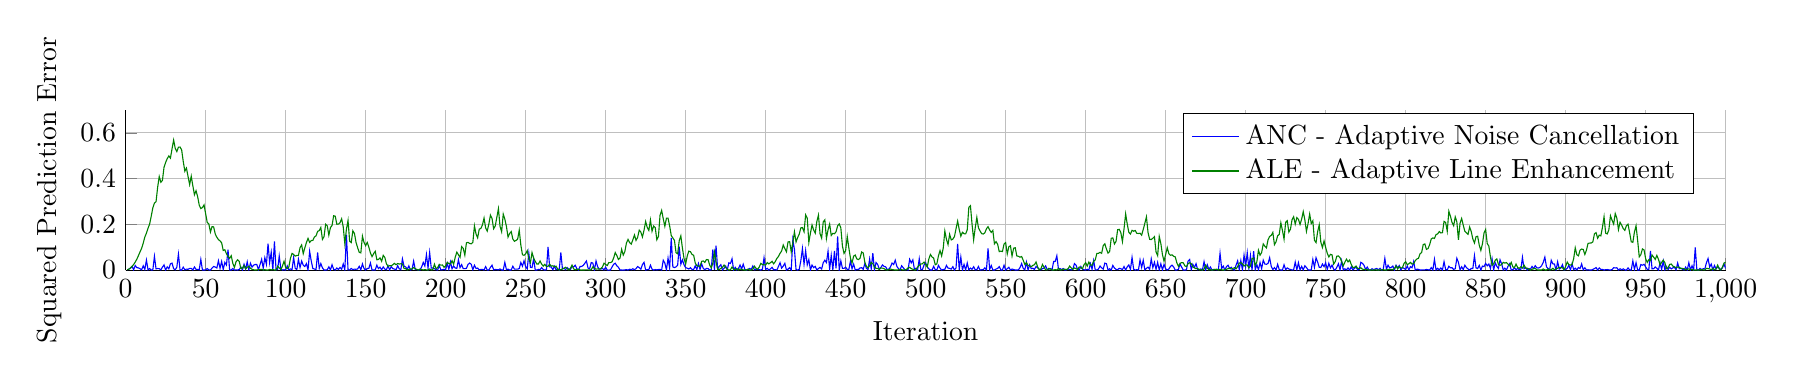
\begin{tikzpicture}

\begin{axis}[%
width=8in,
height=0.8in,
scale only axis,
xmin=0,
xmax=1000,
xlabel={Iteration},
xmajorgrids,
ymin=0,
ymax=0.7,
ylabel={Squared Prediction Error},
ymajorgrids,
axis x line*=bottom,
axis y line*=left,
legend style={draw=black,fill=white,legend cell align=left}
]
\addplot [color=blue,solid]
  table[row sep=crcr]{1	0.000986635785864219\\
2	0.00394264934276108\\
3	0.00885637463565566\\
4	0.0157084194356844\\
5	0.0012605448333739\\
6	0.0199238208109927\\
7	0.0105892237912251\\
8	0.00970744083176815\\
9	0.00572929642281373\\
10	0.00127397236933246\\
11	0.0187641330669286\\
12	0.00281861190218193\\
13	0.0438006541154544\\
14	0.000809030786740652\\
15	0.00665643828144124\\
16	0.000176153212723391\\
17	0.000722206950375272\\
18	0.0602242988362365\\
19	0.00529856351054134\\
20	0.00669996994245621\\
21	0.00638711378423228\\
22	0.000771853439814306\\
23	0.0127436615070615\\
24	0.0225237591458823\\
25	8.95726489536196e-06\\
26	0.0142385158886845\\
27	0.00542862284055068\\
28	0.0274234832127544\\
29	0.0304726076085255\\
30	0.00575949595179903\\
31	0.00116964087720408\\
32	0.0128971390382037\\
33	0.0695718698542331\\
34	0.000345113452149632\\
35	2.97583716612655e-05\\
36	0.0126208124607136\\
37	0.00119096562599838\\
38	0.00429737411137758\\
39	0.00335118534708105\\
40	0.00716070279686857\\
41	0.00727068125374146\\
42	0.000307262453439321\\
43	0.0137047800658569\\
44	0.00282862648233609\\
45	0.00281957601168213\\
46	0.00125766973893199\\
47	0.0464878287162564\\
48	4.57157849944859e-05\\
49	0.000168772268055978\\
50	0.000774024393276305\\
51	0.00658406457780813\\
52	0.000125064861875663\\
53	0.000130112886919977\\
54	0.00864229750630629\\
55	0.0159720045882984\\
56	0.0131682936697162\\
57	0.0090838036921947\\
58	0.0406020676153786\\
59	0.007912549268188\\
60	0.0378767638090336\\
61	0.00306466452236721\\
62	0.033459329332088\\
63	0.0220260203238255\\
64	0.0888511050929133\\
65	2.04124811287403e-05\\
66	0.000247503726767766\\
67	0.00702901244838991\\
68	0.000155287402971255\\
69	0.000919074767123085\\
70	0.000293956589719006\\
71	0.00234189979590632\\
72	0.0129815627117424\\
73	9.62309693276839e-05\\
74	0.0254686273025368\\
75	0.00401050748450727\\
76	0.0361377079208529\\
77	0.000619312412398422\\
78	0.0298727791250182\\
79	0.0128805407793876\\
80	0.0214875279537171\\
81	0.0246763055838764\\
82	0.0241670043019927\\
83	0.00172045834739806\\
84	0.0240152859368831\\
85	0.0469768783452578\\
86	0.00832941084033142\\
87	0.0539813352752297\\
88	0.0252503258312072\\
89	0.115786137220792\\
90	0.0328567060601397\\
91	0.0781825546316058\\
92	0.00041948558257757\\
93	0.1252692670887\\
94	0.00111974415045526\\
95	0.00245873436578155\\
96	0.0619186453774067\\
97	0.00587072110679977\\
98	0.000125105996746423\\
99	0.0014116155135091\\
100	7.11242073138543e-05\\
101	0.0181610842615675\\
102	0.00118305030775922\\
103	0.00515542002307458\\
104	0.00205384570281352\\
105	0.0550107262897427\\
106	0.00736603523621223\\
107	0.0023269055918173\\
108	0.0475741153467194\\
109	0.011340760187443\\
110	0.0395553806715877\\
111	0.0213534582783228\\
112	0.0154612623945079\\
113	0.0282011734084322\\
114	0.000661318782565795\\
115	0.0821416178563193\\
116	0.0403143464310302\\
117	0.00661195176955667\\
118	0.00470850749761054\\
119	0.00185069498240674\\
120	0.0768833142918168\\
121	0.00763959077744209\\
122	0.0283316908548818\\
123	0.00972966910062274\\
124	0.000469783525731509\\
125	6.36902659392701e-05\\
126	0.0012166946060844\\
127	0.0138326720357313\\
128	0.00037741851375222\\
129	0.0233543224521954\\
130	0.0032644708437982\\
131	0.000339022297684614\\
132	0.00918872938062774\\
133	0.00247851732502414\\
134	0.0117613546066365\\
135	0.00372885687835228\\
136	0.0269089958665716\\
137	0.00105240528156839\\
138	0.154688965861569\\
139	0.000950318773434126\\
140	0.000708189319057092\\
141	0.00694535919539114\\
142	0.00207774204210339\\
143	0.00405302109844384\\
144	0.00354338347499521\\
145	0.00484065811437652\\
146	0.0163718982721106\\
147	0.00114157422529363\\
148	0.0269685912156865\\
149	0.00654845212160203\\
150	2.11537809464108e-06\\
151	0.00674698367990745\\
152	0.00735661349495012\\
153	0.0308334360650446\\
154	0.00019219853995476\\
155	0.000624478577947927\\
156	0.000455117393371278\\
157	0.0215110774268121\\
158	0.00662605125226341\\
159	0.0125842367172043\\
160	0.000903978977889658\\
161	0.0140408525874281\\
162	0.00426036929039156\\
163	0.0013373991783078\\
164	0.0188648284114259\\
165	0.000236114952382343\\
166	0.0155538570103688\\
167	0.00625672736859844\\
168	0.0043622542833737\\
169	0.000976060458216981\\
170	0.0189573154766175\\
171	0.00575373671289674\\
172	0.00119809453573357\\
173	0.0490854419913601\\
174	0.0168895423569975\\
175	0.0137648930766898\\
176	0.00316728905662458\\
177	0.0184551352449776\\
178	0.000321156473849071\\
179	0.00277785951877279\\
180	0.0392139201182255\\
181	0.00282763825162243\\
182	0.00182134191417503\\
183	0.000852220043994202\\
184	0.000297377343161396\\
185	0.0134177598088746\\
186	0.0333918463029821\\
187	0.0177086048940856\\
188	0.0676994564541842\\
189	0.00825369075984875\\
190	0.0770251997913325\\
191	0.00922172482481985\\
192	0.00916969165772009\\
193	0.00605703038562923\\
194	0.00158134762625695\\
195	6.77016857317964e-05\\
196	0.0204999232658923\\
197	0.000680342548477276\\
198	0.00148088402223995\\
199	0.0033737772119294\\
200	0.000597147850801516\\
201	0.0295997918548524\\
202	0.0028008580948254\\
203	0.0361550021695272\\
204	0.00582284440372931\\
205	0.0177823069804247\\
206	0.00883770616457795\\
207	0.0074934822601744\\
208	0.0452181074118924\\
209	0.0106959461418465\\
210	0.0235268595612091\\
211	0.00636176419837192\\
212	0.00648794329880858\\
213	0.00737004300088809\\
214	0.0248581239949839\\
215	0.0305257646944547\\
216	0.0253865540453521\\
217	0.00142829252577517\\
218	0.0210804715566955\\
219	0.00667500585022641\\
220	0.00869211103894656\\
221	0.000515357133687416\\
222	0.00272013665888607\\
223	0.00329519552569132\\
224	0.000246672225663202\\
225	0.0151575446083124\\
226	8.19401667738101e-06\\
227	0.000498492936109527\\
228	0.0116771369293351\\
229	0.0214607915491467\\
230	0.000806553689142056\\
231	0.00286470389161256\\
232	0.00194899301744811\\
233	0.00104115092441055\\
234	0.00491257383205808\\
235	9.79718817067421e-05\\
236	0.000243065335109445\\
237	0.0336404984910928\\
238	0.00164446195553912\\
239	0.00414938175444634\\
240	0.000233121838276371\\
241	0.00054795484055497\\
242	0.0168914123147108\\
243	0.00406189057418515\\
244	0.00424286692829463\\
245	0.00409234744640909\\
246	0.00650716016818871\\
247	0.0332024088195594\\
248	0.0171047388612311\\
249	0.040559816296962\\
250	0.0146469753758916\\
251	0.00513499959304226\\
252	0.0734804398204768\\
253	0.0120208367461391\\
254	0.0113197718263265\\
255	0.0489272923199531\\
256	5.53135538498623e-05\\
257	6.40630610768758e-05\\
258	0.00330025409669779\\
259	0.00148973442713983\\
260	0.0106376278049349\\
261	0.00245446671095767\\
262	4.73679355358936e-05\\
263	0.00161353175000448\\
264	0.101273858817055\\
265	0.0140783050530005\\
266	0.0132576143906019\\
267	0.00153705680091184\\
268	0.0168942089882575\\
269	0.00159190237098449\\
270	0.00504119904168183\\
271	0.000586506938123073\\
272	0.0769022791325647\\
273	0.0049537510966466\\
274	0.00775559950130514\\
275	0.00194625708558635\\
276	0.0109868487627397\\
277	0.00367084515898661\\
278	0.0020129241879253\\
279	0.0162208576149772\\
280	0.0137369849733521\\
281	0.0211077961872355\\
282	0.00558926449303668\\
283	1.6464316196899e-05\\
284	0.0156283262904777\\
285	0.0158957217404304\\
286	0.0205858465465557\\
287	0.0295768640696163\\
288	0.0396798728981216\\
289	0.00853366240601832\\
290	0.00540830620320314\\
291	0.033018343613255\\
292	0.0304306547029992\\
293	3.10196387622084e-08\\
294	0.0397201676333331\\
295	0.0144140623730408\\
296	0.00419175323671914\\
297	0.00448185675181755\\
298	0.00702614856436064\\
299	0.00110317409079426\\
300	0.0124440945473084\\
301	4.7336718954208e-05\\
302	2.57028681400028e-05\\
303	0.000106045317626341\\
304	0.0135464936870557\\
305	0.0253157486315755\\
306	0.0299998874789346\\
307	0.018570250104713\\
308	0.0117822875606835\\
309	0.000232458416130835\\
310	7.06331090604118e-05\\
311	4.34917880976854e-05\\
312	0.000493786655451447\\
313	0.00209332744210011\\
314	6.33845701781858e-06\\
315	0.00377341956459579\\
316	0.00144244858767203\\
317	0.00569205482344934\\
318	0.00170583041259822\\
319	0.00617318680366598\\
320	0.015372065924532\\
321	0.0106432004995643\\
322	0.00340304352497313\\
323	0.0241929032825733\\
324	0.0337927255539654\\
325	2.29036587110158e-06\\
326	0.00182209663894011\\
327	0.00170902509414121\\
328	0.0213046630353109\\
329	0.00376342177188011\\
330	0.000180588928335023\\
331	0.00230996238215359\\
332	0.000897361382896648\\
333	0.00221089463809666\\
334	0.0031040008439914\\
335	0.000115893865776731\\
336	0.0430736336595949\\
337	0.0304826196746853\\
338	0.000728623895087639\\
339	0.0519960225977006\\
340	0.00804200961449122\\
341	0.140445557150897\\
342	0.0138093656938474\\
343	0.0109632274321883\\
344	0.0137566057351353\\
345	0.021197734344565\\
346	0.102553972278132\\
347	0.0253906056823893\\
348	0.0447164020293579\\
349	0.0232493388062389\\
350	0.0102655631691967\\
351	0.00819195182917725\\
352	0.00455198455273308\\
353	0.0104071175885201\\
354	0.00263440594885222\\
355	0.00276242431857184\\
356	0.0184157575241905\\
357	0.0019870513358324\\
358	0.0288074673633775\\
359	0.00270077128616477\\
360	0.0273977122611628\\
361	0.00762311621514521\\
362	0.00151848122196824\\
363	0.00703300183627435\\
364	0.00650491560561162\\
365	0.000107238948325999\\
366	0.00129724179006489\\
367	0.089802135602975\\
368	0.000715377545710117\\
369	0.106749341905659\\
370	0.00403714978837018\\
371	0.0157532442138971\\
372	0.0235387736606012\\
373	0.00027989182848627\\
374	0.00766055981146411\\
375	0.0174780569616289\\
376	0.000236266370802925\\
377	0.0315747072246476\\
378	0.029097585169937\\
379	0.0494127626173825\\
380	0.000631523607300933\\
381	0.0118481597983318\\
382	0.000223454565155297\\
383	0.00613299055538471\\
384	0.0221992132588379\\
385	0.00504844039539135\\
386	0.0255138291976885\\
387	0.00312172253597758\\
388	1.89835063412605e-05\\
389	0.00219008399855425\\
390	0.00728510910046507\\
391	0.00315697107307067\\
392	0.0178078420490909\\
393	0.00134961382721221\\
394	0.00292009524623769\\
395	0.00344619730839487\\
396	0.00244337945320282\\
397	2.83554236116993e-06\\
398	0.00384131495234512\\
399	0.0538589111169449\\
400	0.00266160000711889\\
401	0.00725174511482355\\
402	4.86122684716553e-06\\
403	0.00508802935280465\\
404	0.0119942285968692\\
405	0.00147893461955511\\
406	0.00161478012536344\\
407	0.000360638123280208\\
408	0.0154598405451951\\
409	0.0322498500525052\\
410	0.00847101367519636\\
411	0.0176640476953157\\
412	0.0293158039208963\\
413	2.01737138163919e-05\\
414	0.00382660421576798\\
415	0.0105396596851566\\
416	0.00020582846387852\\
417	0.133054793134052\\
418	0.0903521896841805\\
419	0.00214949220951932\\
420	0.000106173225095851\\
421	0.00313731007554933\\
422	0.0410379634981064\\
423	0.0943551009330556\\
424	0.0253834341563762\\
425	0.0847627001546714\\
426	0.0225969573142994\\
427	0.0456063794943234\\
428	0.000340464769977014\\
429	0.0218106676189823\\
430	0.0105670366692494\\
431	0.0160925813195453\\
432	5.77108396991808e-07\\
433	0.00660979666510387\\
434	0.0119261572417531\\
435	0.004826561710313\\
436	0.0322282602498643\\
437	0.0430657161852808\\
438	0.032912375686933\\
439	0.0824384583147645\\
440	0.00340326952286744\\
441	0.0638861350239254\\
442	6.22999062039784e-05\\
443	0.0840454355769801\\
444	0.00756563941444837\\
445	0.147577594334632\\
446	0.000221894294166436\\
447	0.0399779055029367\\
448	0.00772275071845888\\
449	0.00754916058697115\\
450	0.0125806482042418\\
451	0.0024760878927145\\
452	0.00233524090243755\\
453	0.0390019796267494\\
454	0.005944151940052\\
455	0.0260688673213836\\
456	0.000219654756414474\\
457	0.00288669286006889\\
458	0.00204007756241234\\
459	0.00940314145971794\\
460	0.0104606128271499\\
461	0.00348314626601728\\
462	0.0286088504634517\\
463	0.00720260640713261\\
464	0.00235196492273629\\
465	0.0485120263747638\\
466	0.00529021082066565\\
467	0.0741254444110785\\
468	5.05118617210214e-06\\
469	0.0328898379705231\\
470	0.0245134136586208\\
471	0.00529770595450543\\
472	0.0106393699199637\\
473	0.0223599771734016\\
474	0.0161399167580108\\
475	0.0140497874298391\\
476	0.00194128512871698\\
477	0.00423306659292713\\
478	0.0134890237648994\\
479	0.030616384681614\\
480	0.0241071945875636\\
481	0.0431402386072958\\
482	0.0164172382857554\\
483	0.00626676435176438\\
484	0.000682929301576132\\
485	0.0188520067555648\\
486	0.0104702856983094\\
487	0.00137239224679826\\
488	0.00217286162660121\\
489	5.32232596043372e-05\\
490	0.0472570402650871\\
491	0.0315765352600603\\
492	0.0446302716117797\\
493	0.00330059102802852\\
494	0.00824291616023502\\
495	4.22830834860425e-07\\
496	0.0494947560831573\\
497	0.00192756044161873\\
498	0.00196211792750299\\
499	0.0225508916671334\\
500	0.031980174218848\\
501	0.0140563311943861\\
502	0.00543502504916628\\
503	1.90674937554394e-05\\
504	0.000186358101369945\\
505	0.0163787073520048\\
506	0.00195361133601601\\
507	0.000674690338587829\\
508	0.0205326633273322\\
509	0.00798529392637406\\
510	0.000260494291764686\\
511	0.00243951565919122\\
512	0.00315095694996699\\
513	0.0203812649372224\\
514	0.00853649084152569\\
515	0.00746086465157584\\
516	0.00420612678221062\\
517	0.0148775250882379\\
518	0.000591798127530651\\
519	0.00955198266656682\\
520	0.114308664820426\\
521	0.000696542559601777\\
522	0.0564564955111076\\
523	1.20607251054324e-07\\
524	0.0246885211009707\\
525	0.000368037094052932\\
526	0.0310826367056789\\
527	0.00087883516064485\\
528	0.00860193779192913\\
529	0.00338179522639953\\
530	0.0144580052468705\\
531	0.00108143739097979\\
532	0.00142222564991991\\
533	0.0155531513642635\\
534	4.93539498920769e-05\\
535	0.00134890306554174\\
536	0.00151050274711192\\
537	0.0102519874892416\\
538	0.00013153572757733\\
539	0.0948348003138718\\
540	0.00272385803267812\\
541	0.0200648105174361\\
542	0.0002006697675515\\
543	0.000126648148483442\\
544	0.00432996079754037\\
545	0.00714246128054442\\
546	0.0150394602879107\\
547	0.000408502489015446\\
548	2.9669252926671e-05\\
549	0.0214237946973844\\
550	5.00155786743991e-05\\
551	0.00587720823056195\\
552	0.0121714496714736\\
553	0.000224564506871128\\
554	0.00432741599705725\\
555	0.00229653518465741\\
556	0.000399514357433151\\
557	0.000244066419310831\\
558	0.00104274711707985\\
559	0.0112468487202022\\
560	0.0284751160977908\\
561	0.00770408199896097\\
562	0.00110765752366632\\
563	0.0348648276042366\\
564	4.97545674569175e-06\\
565	0.022889665307898\\
566	0.00599602873438033\\
567	0.00821355143118291\\
568	0.00220156982227422\\
569	0.0159702477468491\\
570	0.00960862282941975\\
571	0.00373327680660391\\
572	0.000819492426679046\\
573	0.00648153356557321\\
574	0.00869578358817569\\
575	0.0182542085223527\\
576	0.00224578674464427\\
577	0.00325678883399286\\
578	0.00672542034816176\\
579	0.00105709380981771\\
580	0.03743503939143\\
581	0.0378344134509999\\
582	0.0626963893095184\\
583	0.00484386190282624\\
584	0.00669949269518087\\
585	0.00204005546965118\\
586	0.00662722049689957\\
587	1.60241242014025e-05\\
588	0.000684014057048492\\
589	0.00481181599802989\\
590	0.00204769580551633\\
591	0.000790977306578494\\
592	0.00319186720876508\\
593	0.0281712034950031\\
594	0.0215096297830973\\
595	0.00224309531660696\\
596	0.000206174886659293\\
597	0.0153713726819869\\
598	0.00399053883656157\\
599	0.0013229565672695\\
600	0.000120630564614319\\
601	0.00357599364727959\\
602	7.87954617411435e-05\\
603	0.0279604767368654\\
604	0.00364318507241058\\
605	0.0419414569790714\\
606	0.000596958330071647\\
607	0.000549896580146255\\
608	0.00448096971349684\\
609	0.0175274996609961\\
610	0.0098608551425635\\
611	0.00424170686365287\\
612	0.0304372646601643\\
613	0.0277769954241606\\
614	3.04074778897589e-07\\
615	0.00544456918696933\\
616	0.000516345253805703\\
617	0.0201977011265629\\
618	0.00883822900282527\\
619	0.0032503329528322\\
620	0.00178994955939062\\
621	0.00760321319180753\\
622	0.00598131265285443\\
623	0.00233378707809592\\
624	0.0153351927054063\\
625	0.000153921082067452\\
626	0.0142794669104485\\
627	0.0225414253768853\\
628	0.0024750284457372\\
629	0.0553463907042274\\
630	0.00359490178935644\\
631	0.000271131315357666\\
632	0.00194896937791566\\
633	2.3741372702008e-06\\
634	0.044681959829127\\
635	0.0114907589207284\\
636	0.0432126719653382\\
637	0.000821914898325398\\
638	0.00747032218883774\\
639	0.0130614701006153\\
640	0.00316333896500048\\
641	0.0488198529495758\\
642	0.0106427767037383\\
643	0.0340326449050708\\
644	0.00335954475706951\\
645	0.0334507357315676\\
646	0.000561560036992275\\
647	0.0275634309891187\\
648	0.000798749517775652\\
649	0.0248566683457671\\
650	0.00514449396313266\\
651	0.000228388253435886\\
652	0.00455950653607176\\
653	0.0158217121034157\\
654	0.021592151112995\\
655	0.013493912620215\\
656	0.000344668504818963\\
657	4.68083332537746e-05\\
658	0.00340072593343264\\
659	0.0268920489215345\\
660	0.0131018551228399\\
661	9.89816298385221e-05\\
662	3.86087312020809e-05\\
663	0.000845634105785164\\
664	0.0390074940922852\\
665	0.0463747364783935\\
666	0.00172370816956038\\
667	0.0255814965791501\\
668	0.0117899057583734\\
669	0.0279967528410641\\
670	0.00154157848928195\\
671	0.00259151539064582\\
672	0.00485648120961841\\
673	0.000268549185770551\\
674	0.0367222168780094\\
675	0.000348512053123545\\
676	0.0233619922993774\\
677	0.00315249894828547\\
678	0.0134984918548077\\
679	8.78279239924572e-05\\
680	0.0028969219174501\\
681	0.00228605425065355\\
682	0.00106189375920044\\
683	0.00283411232669083\\
684	0.0735018768134007\\
685	0.00722355457164992\\
686	0.0174116306051738\\
687	0.00025680607537769\\
688	0.0147935949467859\\
689	0.021101686188377\\
690	0.00730507465855082\\
691	0.0122810640838183\\
692	0.00268450608093025\\
693	0.000137639825185166\\
694	0.0211152540330262\\
695	0.0406358758822373\\
696	0.00188226891585178\\
697	0.0416666642881951\\
698	0.000531294541468825\\
699	0.0658625934402545\\
700	0.0168775168619939\\
701	0.0759670284736007\\
702	0.0078426390100546\\
703	0.0639355893471729\\
704	0.000101408388251338\\
705	0.0831056303872603\\
706	0.00193753400697931\\
707	0.0234333758420414\\
708	0.00112955413171272\\
709	0.0328338366207815\\
710	0.0060345104174419\\
711	0.0432813115971497\\
712	0.0265198704718756\\
713	0.0252260426966876\\
714	0.0290240126221982\\
715	0.0540402410583876\\
716	0.0166179642266378\\
717	0.00263426129416561\\
718	0.0107449272598287\\
719	8.63116557544096e-06\\
720	0.0252386871538406\\
721	0.00186915278922952\\
722	0.000479522173363441\\
723	0.000138266673967405\\
724	0.0229366583322393\\
725	0.00175418910181453\\
726	0.00943217928286258\\
727	0.00484664022479967\\
728	0.0025444585976791\\
729	0.000512942151712897\\
730	0.00142935837327358\\
731	0.0350180441270523\\
732	0.000952988306320521\\
733	0.0319216467618171\\
734	0.000628672798403354\\
735	0.0158979273469661\\
736	0.00085620715182149\\
737	0.0189347589882319\\
738	0.0110974171314029\\
739	0.000882296974739401\\
740	0.000255242820525863\\
741	0.000799536756505775\\
742	0.0464395736784649\\
743	0.0117059224104486\\
744	0.0539058067458675\\
745	0.0349356624686018\\
746	0.0120560977838536\\
747	0.0114162967464463\\
748	0.0263621331124394\\
749	0.0148447891228119\\
750	0.0316207318803499\\
751	0.00257747702764045\\
752	0.029437255629475\\
753	0.00949692757914545\\
754	0.0215191751121429\\
755	0.00404297533432734\\
756	4.643046174798e-05\\
757	0.0125453192172437\\
758	0.0276180534912735\\
759	0.00064707921085046\\
760	0.0404007821067375\\
761	0.000685902187271107\\
762	0.00559589377002391\\
763	0.000469415471954841\\
764	0.00942443978846106\\
765	7.03682648679335e-05\\
766	0.0140596668071206\\
767	0.000874606886822472\\
768	0.00762554493107278\\
769	0.0134747291632053\\
770	0.000503129197262285\\
771	0.00317299726302695\\
772	0.0337910130813887\\
773	0.0296476634659161\\
774	0.0206833708880561\\
775	0.00223493981305485\\
776	0.0132876511602529\\
777	0.00041381455143779\\
778	0.000555697297719617\\
779	0.00568416353830165\\
780	0.0017578255279298\\
781	0.00478214641009504\\
782	0.00722149470172853\\
783	0.000619997928977272\\
784	0.00761493416079639\\
785	7.99045235301898e-05\\
786	0.00302198825948439\\
787	0.0512410982543579\\
788	0.00354372411163376\\
789	0.0211816708829928\\
790	0.00954384002234368\\
791	0.0115248039199232\\
792	0.0175644431463106\\
793	0.000543410691720973\\
794	0.0208671034260445\\
795	0.0098686999903917\\
796	0.0196056834968098\\
797	0.000412944818277495\\
798	0.0109259983664992\\
799	0.00757643676672422\\
800	0.00207204860752634\\
801	0.0180997780249068\\
802	0.000161374346166724\\
803	0.0152172363398671\\
804	0.0102398579379328\\
805	0.0370586763492446\\
806	0.000333799927123103\\
807	0.00365458952154541\\
808	0.00326802123167251\\
809	2.51803881974784e-05\\
810	0.000697651259459471\\
811	0.000713921816731418\\
812	0.000885219426160575\\
813	0.00252003343899289\\
814	0.00131226753265341\\
815	0.000353577449321758\\
816	0.0110591396439827\\
817	2.6744337908227e-06\\
818	0.0469771844263134\\
819	1.31413182725348e-06\\
820	0.00754899945461914\\
821	0.00107529758677994\\
822	0.00914536524402185\\
823	0.000682482835503861\\
824	0.0366717872108958\\
825	0.00277463706681293\\
826	0.000392215918075919\\
827	0.0167782544995114\\
828	0.00995137767863267\\
829	0.010083389271374\\
830	0.00293614147681628\\
831	0.00583166255044097\\
832	0.0513308204858947\\
833	0.0331159085518892\\
834	0.00129399633304702\\
835	0.0142166001286464\\
836	0.0020572892429372\\
837	0.0211976399960476\\
838	0.0106724116110986\\
839	0.00489986245157518\\
840	1.0940457495022e-05\\
841	0.0068920668259934\\
842	0.00642055282438337\\
843	0.0631558678059435\\
844	0.0091575967600844\\
845	0.00643707817704945\\
846	0.0204684650949708\\
847	4.92915309940431e-05\\
848	0.0174219272200719\\
849	0.0149792131577666\\
850	0.0291719175634467\\
851	0.018540626590573\\
852	0.0265624391929526\\
853	0.00683774092509751\\
854	0.0495708786995823\\
855	0.000459984313119911\\
856	0.0315814335758831\\
857	0.0164392161615843\\
858	0.0069232651711508\\
859	0.0449352338145058\\
860	0.0276894696857064\\
861	0.000669256154379703\\
862	0.00844854639786075\\
863	0.000108234438615397\\
864	0.0167148484067478\\
865	0.027825949622083\\
866	0.000131682857676427\\
867	0.00188807381333693\\
868	0.00918591497843478\\
869	0.00242482114155661\\
870	0.00625484846045269\\
871	0.00204607464343328\\
872	0.00262781388775591\\
873	0.0558028881128885\\
874	0.00587275930710416\\
875	0.0116555459810039\\
876	0.000356388037134527\\
877	0.00661788293119144\\
878	0.00430995556825676\\
879	0.0158955804740827\\
880	0.00647650777188054\\
881	0.0190959393051411\\
882	0.00955472517910295\\
883	0.00895868133122792\\
884	0.0121791335144085\\
885	0.0190267018180385\\
886	0.0337091081570951\\
887	0.0567775557216298\\
888	0.0142974958275627\\
889	0.0065036066754258\\
890	0.00157656707975002\\
891	0.0428835127109415\\
892	0.0270405299422552\\
893	0.0263768844465435\\
894	5.08201480564741e-05\\
895	0.0364077501421101\\
896	0.00440677464339513\\
897	0.00945725921413068\\
898	0.0236430569614931\\
899	0.000123690415179683\\
900	0.00228283802502936\\
901	0.00795158639086217\\
902	0.0213711876553561\\
903	0.00010732054280493\\
904	0.0277243100655181\\
905	0.00222537209284135\\
906	0.00834165321434058\\
907	0.000696250003696828\\
908	0.0111829378802633\\
909	0.00655843300221848\\
910	0.0267944054492523\\
911	0.00103826187496294\\
912	0.0102068859280883\\
913	0.00053453149989607\\
914	0.00138233501635695\\
915	0.00040210961895032\\
916	2.36535010381983e-05\\
917	0.00285229520959767\\
918	0.00623906366797323\\
919	0.0109619503594267\\
920	0.000304233578428456\\
921	0.00916773954915981\\
922	0.00278247290928847\\
923	0.0029390634860949\\
924	1.60752043969124e-05\\
925	0.00192729359653452\\
926	0.00225055442539049\\
927	0.000806812270209154\\
928	0.000476468045259908\\
929	0.00199007537726468\\
930	0.0102360174007557\\
931	0.00928151445659129\\
932	0.0101160785422839\\
933	0.00030661624896989\\
934	0.0056260592076547\\
935	0.00101626249197209\\
936	0.00516113408893847\\
937	0.000600594427241475\\
938	5.07687739253525e-05\\
939	0.00959988138087169\\
940	0.000667094883739358\\
941	0.000334798774112213\\
942	0.0402318679682116\\
943	0.00266066221722307\\
944	0.0324042161019118\\
945	8.32429054916097e-05\\
946	0.000339858873521657\\
947	0.0241356866539626\\
948	0.0212346421754895\\
949	0.0253378037655006\\
950	0.0138523647173283\\
951	0.00250981785546075\\
952	0.00301194955456093\\
953	0.0836756755600999\\
954	0.00504406087672074\\
955	0.00611747553131608\\
956	0.0134391459446695\\
957	0.00767745649297077\\
958	1.9453132388672e-05\\
959	0.031854286644245\\
960	0.00279431982305932\\
961	0.039147861476613\\
962	0.000892964965458962\\
963	0.0155644300626306\\
964	0.00242168897309738\\
965	0.01186205600345\\
966	0.0052757596359166\\
967	0.00957883681153323\\
968	0.0120771724203297\\
969	0.000725960697980537\\
970	0.0310049432046879\\
971	0.00589479018378078\\
972	0.00853249419215862\\
973	0.00363102662412054\\
974	0.00056978893307773\\
975	0.0129637210307948\\
976	4.98407950995016e-05\\
977	0.0321185301705693\\
978	0.0013183736813487\\
979	0.0189552158502786\\
980	2.05135590666119e-05\\
981	0.098666957105404\\
982	0.00180383138692472\\
983	7.26067448251663e-05\\
984	0.00718047130718431\\
985	0.00169094992934624\\
986	0.00603725413219746\\
987	0.004830132220371\\
988	0.0323177849066719\\
989	0.0504889549004673\\
990	0.0136951289394792\\
991	0.0261839818885803\\
992	0.000305615018129508\\
993	0.0200299822253926\\
994	0.00498797489491953\\
995	0.0133784602825721\\
996	0.00895717653283971\\
997	0.00105483409881511\\
998	0.00999596724178313\\
999	0.0263045929697207\\
1000	0.00643167758596159\\
};
\addlegendentry{ANC - Adaptive Noise Cancellation};

\addplot [color=black!50!green,solid]
  table[row sep=crcr]{1	0.000986635785864219\\
2	0.00394264934276108\\
3	0.00885637463565566\\
4	0.0157084194356844\\
5	0.0244717418524232\\
6	0.0351117570558743\\
7	0.0475864737669902\\
8	0.0633161666811966\\
9	0.0796198361318386\\
10	0.0952962308840211\\
11	0.117788618512144\\
12	0.144733798919446\\
13	0.161525651144512\\
14	0.183171174376491\\
15	0.201179884465927\\
16	0.235673299072756\\
17	0.272339649434188\\
18	0.29323574897421\\
19	0.299065979250237\\
20	0.361882663031675\\
21	0.409312863400909\\
22	0.384047572786942\\
23	0.392414941711003\\
24	0.450309381540812\\
25	0.471119575606435\\
26	0.48737456782625\\
27	0.499320613621541\\
28	0.489833076856592\\
29	0.530500320886282\\
30	0.5686518358587\\
31	0.532331226443785\\
32	0.518473469331292\\
33	0.537460348473857\\
34	0.538211325308672\\
35	0.526235407601997\\
36	0.475463255291207\\
37	0.432440255927798\\
38	0.4461270351255\\
39	0.409864468587289\\
40	0.374029757936215\\
41	0.410477577557875\\
42	0.36918970690247\\
43	0.329556808828088\\
44	0.347272580608485\\
45	0.32117687354237\\
46	0.283990034903177\\
47	0.269058353611844\\
48	0.273440438164021\\
49	0.285116388889057\\
50	0.246719101721121\\
51	0.207898645085437\\
52	0.202260505229042\\
53	0.166231287215613\\
54	0.190123036076114\\
55	0.189081435868908\\
56	0.158014386237692\\
57	0.143599591083471\\
58	0.133573877462677\\
59	0.127428674091172\\
60	0.119614754168082\\
61	0.0857292545527413\\
62	0.0889075185890149\\
63	0.0715825054543774\\
64	0.0601157344019595\\
65	0.0513508273482877\\
66	0.0627264010054099\\
67	0.0291750449370511\\
68	0.0118555945171372\\
69	0.0363475244677917\\
70	0.045137092023101\\
71	0.0375682508502001\\
72	0.0071911273390196\\
73	0.00813540542551852\\
74	0.0201906605130298\\
75	0.00498317301818962\\
76	0.0125013811179398\\
77	0.0164913660611397\\
78	0.00793986505306365\\
79	0.00343937183674032\\
80	0.00124209187404757\\
81	0.000216208329455021\\
82	0.000712696652400544\\
83	0.00161334935995707\\
84	0.00213130097306363\\
85	0.00304233601721613\\
86	0.000273782263463404\\
87	0.00171430526002042\\
88	0.000128586120876438\\
89	3.84031546894147e-06\\
90	0.00315203256520743\\
91	0.000721260422723975\\
92	0.00264912220006151\\
93	0.000124458165930989\\
94	0.000149887446842824\\
95	0.017022614992866\\
96	0.00937735267754249\\
97	0.00212835063486533\\
98	0.0174891708507811\\
99	0.0381901391036194\\
100	0.012372140686644\\
101	0.00636200761901439\\
102	0.0131893173324762\\
103	0.0515132191901975\\
104	0.0730074122594794\\
105	0.0682152512353694\\
106	0.0610428222304548\\
107	0.0640067688671438\\
108	0.0642734128423494\\
109	0.0977423299119522\\
110	0.110149018232092\\
111	0.0718076236084536\\
112	0.0972925470848119\\
113	0.120805384892249\\
114	0.138585921840012\\
115	0.12097059845765\\
116	0.129061016192223\\
117	0.129891513186261\\
118	0.144735316423889\\
119	0.149755621181448\\
120	0.169209109559942\\
121	0.172503954447105\\
122	0.186194949966095\\
123	0.134089460740299\\
124	0.146577646936905\\
125	0.200645408490419\\
126	0.193635435599611\\
127	0.152687193212756\\
128	0.185889607269837\\
129	0.195182224571202\\
130	0.237536148714457\\
131	0.236006032266295\\
132	0.2004736746526\\
133	0.201046990511297\\
134	0.207209160406386\\
135	0.224431290989433\\
136	0.188890843305328\\
137	0.115129533337159\\
138	0.178965843550741\\
139	0.21691772156947\\
140	0.126286884500938\\
141	0.120015819778403\\
142	0.17165052325773\\
143	0.160429639731228\\
144	0.121026148375022\\
145	0.0979101720579266\\
146	0.0772269548538773\\
147	0.0752098332661802\\
148	0.148300930804931\\
149	0.12075297579079\\
150	0.106364326078087\\
151	0.120781287440966\\
152	0.100869398228279\\
153	0.0745502675638662\\
154	0.0591153535572801\\
155	0.0718197978806773\\
156	0.0822059048585231\\
157	0.0449629132983402\\
158	0.0466878593902391\\
159	0.0532365639061773\\
160	0.0385515394308937\\
161	0.0643608519009155\\
162	0.0550943851421962\\
163	0.0271312224974754\\
164	0.016352029293355\\
165	0.0194450155231395\\
166	0.018853310766426\\
167	0.0231616043371191\\
168	0.0294345260555496\\
169	0.0233146997337533\\
170	0.0285154114539286\\
171	0.0264549574975232\\
172	0.0275365142273254\\
173	0.0269285187029132\\
174	0.00688864205300433\\
175	0.00593437769526723\\
176	0.000451397064978999\\
177	0.00312519147574745\\
178	0.00482679513343046\\
179	0.00489294401276036\\
180	0.0113394041450996\\
181	0.00637625417755734\\
182	0.00281636482449525\\
183	4.96260231556338e-05\\
184	0.00438833878469726\\
185	0.00205586541744545\\
186	0.000623196720637001\\
187	0.00187442006568334\\
188	0.000595828816121693\\
189	0.000303490650502472\\
190	0.00485914366777304\\
191	0.00044513158061191\\
192	0.00198874318353236\\
193	0.0258134583759807\\
194	0.00603429871543773\\
195	0.0103374189897564\\
196	0.0247269430065183\\
197	0.0214563823025285\\
198	0.0221460169902619\\
199	0.0124211760412809\\
200	0.0182586977808381\\
201	0.0337389808175739\\
202	0.02851021041923\\
203	0.0269178671455115\\
204	0.0409670416600899\\
205	0.0254968034476332\\
206	0.0564288524131958\\
207	0.0786368753336259\\
208	0.066962629515082\\
209	0.0552673700972248\\
210	0.102426060483725\\
211	0.0948770163960479\\
212	0.0654135357485515\\
213	0.119335951747956\\
214	0.120981483189963\\
215	0.116480926219243\\
216	0.114869888860177\\
217	0.120983537540125\\
218	0.193156815355351\\
219	0.157782002397551\\
220	0.141084727678418\\
221	0.178757684616996\\
222	0.182242548049563\\
223	0.196903430849975\\
224	0.22750609717223\\
225	0.184298529759474\\
226	0.170656548650007\\
227	0.201061624032419\\
228	0.240267996185046\\
229	0.225711553637568\\
230	0.180673866420467\\
231	0.192912407526272\\
232	0.230669439809248\\
233	0.268484010402149\\
234	0.191204571446197\\
235	0.167471357102061\\
236	0.245015074880081\\
237	0.222790153453467\\
238	0.19074751860563\\
239	0.144243497925392\\
240	0.160155790104324\\
241	0.168376908798354\\
242	0.135777361738494\\
243	0.125840197049093\\
244	0.129601997134613\\
245	0.135062627644577\\
246	0.174873357474819\\
247	0.109251735812584\\
248	0.0672462771429152\\
249	0.0642799848852176\\
250	0.0714177675502619\\
251	0.0851343462943177\\
252	0.048868068577449\\
253	0.0332158798213729\\
254	0.0765715119069338\\
255	0.0522308127517336\\
256	0.0381928870252203\\
257	0.0265349897960173\\
258	0.0264162916983629\\
259	0.0398592335457166\\
260	0.0261664880962429\\
261	0.0175942020248634\\
262	0.025066341529301\\
263	0.015454317085981\\
264	0.0159869427436538\\
265	0.0257696691211742\\
266	0.0171042475769634\\
267	0.0189073391555778\\
268	0.0142787704338044\\
269	0.0171425313108282\\
270	0.00412635380937665\\
271	0.000559255544360664\\
272	0.00217833305133767\\
273	0.00514001373400503\\
274	0.00840104641616173\\
275	0.01221104066202\\
276	0.00527970707773192\\
277	0.000800608153874982\\
278	0.00761863970478217\\
279	0.0217507218791515\\
280	0.0052157254691602\\
281	0.00152575114390875\\
282	0.00304588581379432\\
283	0.00426275220650597\\
284	0.000242468070161426\\
285	3.86398937165835e-05\\
286	0.000230685333704153\\
287	0.000599279800651977\\
288	0.000919221042563011\\
289	0.000673791671061676\\
290	0.000260990775555537\\
291	0.00176667769913323\\
292	0.01403615120962\\
293	0.00765616271209831\\
294	0.00389268665512788\\
295	0.00523426235070843\\
296	0.00407501562397361\\
297	0.00615450942796492\\
298	0.0135134343681404\\
299	0.0301177588964612\\
300	0.0244124905492157\\
301	0.0197885029162982\\
302	0.0328887590267922\\
303	0.0323300872163124\\
304	0.0362564178854664\\
305	0.0527306148323484\\
306	0.0764953366974595\\
307	0.0633133752574472\\
308	0.0462028853033742\\
309	0.0528775123326059\\
310	0.0905230801314736\\
311	0.0655487337699338\\
312	0.0810059226165477\\
313	0.118357076811809\\
314	0.134144492534038\\
315	0.119983553156397\\
316	0.113508299119869\\
317	0.132143502478923\\
318	0.153629721775831\\
319	0.12982689284458\\
320	0.143334415405171\\
321	0.174715383947152\\
322	0.166115449949657\\
323	0.144922999832687\\
324	0.174302856414985\\
325	0.212459354488859\\
326	0.186572989465946\\
327	0.173363438399272\\
328	0.219049843052588\\
329	0.169934273985636\\
330	0.192857104304912\\
331	0.185879046928531\\
332	0.132470209938445\\
333	0.146627925603036\\
334	0.240343666894026\\
335	0.261198370996967\\
336	0.224765401761367\\
337	0.191173215947312\\
338	0.22706807947473\\
339	0.226905832818788\\
340	0.193082023795016\\
341	0.15097854940747\\
342	0.140578886305496\\
343	0.129788430995357\\
344	0.0760391511736219\\
345	0.0711168362790183\\
346	0.128840938169115\\
347	0.149633955829711\\
348	0.0955375153985586\\
349	0.0503297637795756\\
350	0.0264277310475293\\
351	0.0613325795547862\\
352	0.0829368036276822\\
353	0.0803227666041197\\
354	0.0684128265440075\\
355	0.0649808331262676\\
356	0.0308715244602067\\
357	0.0188895886599338\\
358	0.0178799419548787\\
359	0.0163444875200054\\
360	0.0381274829042186\\
361	0.0396752591580575\\
362	0.0336387466403916\\
363	0.0459853477375275\\
364	0.0456989038816794\\
365	0.0225173818616944\\
366	0.00937705246744552\\
367	0.0305417559723558\\
368	0.0795929160350173\\
369	0.0362099280828585\\
370	0.00266100587677017\\
371	0.00264013562901981\\
372	0.00708001847774392\\
373	0.0119652142712564\\
374	0.0219095655679819\\
375	0.0118116595365343\\
376	0.00365007364616222\\
377	3.82723467203816e-05\\
378	0.00153712992443002\\
379	0.0137707035444369\\
380	0.0025970503386365\\
381	0.0014945225105405\\
382	0.00673403997661131\\
383	0.000389061252840371\\
384	0.00458650246536038\\
385	0.00206385917165982\\
386	0.000978091566700175\\
387	8.73294205504928e-05\\
388	5.04253242149692e-05\\
389	0.00421559047120113\\
390	5.72241087545917e-05\\
391	0.000425848457803106\\
392	0.00454194786911969\\
393	0.0169476273345001\\
394	0.0075757562835561\\
395	0.00346537990500778\\
396	0.0131799749394103\\
397	0.0293547692437142\\
398	0.0237670034931651\\
399	0.0231111874127556\\
400	0.0221885232386988\\
401	0.0328283793737011\\
402	0.0270452640352353\\
403	0.032040098611144\\
404	0.0383131969756068\\
405	0.0274923127302957\\
406	0.0370194084670169\\
407	0.0505908895252613\\
408	0.0595322380805423\\
409	0.0731952963516849\\
410	0.0836059851333304\\
411	0.109770351838168\\
412	0.0937892374266293\\
413	0.0799523745043088\\
414	0.123248149834915\\
415	0.124401778420397\\
416	0.0793191139557342\\
417	0.119876090099512\\
418	0.167384360773692\\
419	0.123148944067934\\
420	0.142149904894506\\
421	0.157384987903435\\
422	0.184563189688143\\
423	0.185769133060169\\
424	0.167726259493964\\
425	0.241701384159974\\
426	0.227585419318314\\
427	0.121056246981053\\
428	0.162125074388284\\
429	0.197402673765659\\
430	0.175200780387398\\
431	0.161191485678259\\
432	0.212831377047081\\
433	0.24050304297488\\
434	0.15901959002735\\
435	0.139479595761231\\
436	0.211012241584215\\
437	0.219666955212523\\
438	0.13825513525508\\
439	0.175716423728437\\
440	0.201002947878749\\
441	0.151502404243118\\
442	0.160630978344753\\
443	0.158887020574676\\
444	0.167384931757542\\
445	0.193500754792961\\
446	0.2020063654915\\
447	0.184712518646643\\
448	0.104603402591379\\
449	0.0727874862087752\\
450	0.0853078586548581\\
451	0.146695806631421\\
452	0.0972281955307704\\
453	0.0523490851615888\\
454	0.0310212676488831\\
455	0.0611568790176975\\
456	0.065614485660521\\
457	0.048588453869877\\
458	0.0458462866635821\\
459	0.0516641762104174\\
460	0.0791606299131983\\
461	0.0745249619329255\\
462	0.0344080420227377\\
463	0.0155751075152952\\
464	0.0101533764751404\\
465	0.0189792354222047\\
466	0.0333955036542544\\
467	0.0279159162858606\\
468	0.0138093458282851\\
469	0.00774180427702307\\
470	0.0073429359498328\\
471	0.00266308279946406\\
472	0.00881085903900585\\
473	0.00863726770800252\\
474	0.00596597391622922\\
475	0.00168273796514755\\
476	0.0003063261503568\\
477	0.00206483776412316\\
478	0.00460006390316626\\
479	0.00211016066192799\\
480	0.00110688556731188\\
481	0.000370196446453465\\
482	0.000218948335762564\\
483	0.00124326662273404\\
484	0.00222814453339089\\
485	0.00135278106565111\\
486	0.000684615762366865\\
487	0.000735079122334913\\
488	0.00226611387385335\\
489	0.00924068632654481\\
490	0.0120473162083505\\
491	0.00643908405728801\\
492	0.00349441140306081\\
493	4.15191538591364e-07\\
494	0.00149537907253627\\
495	0.0133643572215922\\
496	0.0212565505622272\\
497	0.0264766782039168\\
498	0.0274060158449118\\
499	0.0349405746453806\\
500	0.0252671941286895\\
501	0.0134388220544021\\
502	0.0487200983298932\\
503	0.068134825208364\\
504	0.057331881305142\\
505	0.0524100663923818\\
506	0.0232294596626147\\
507	0.0269948893128649\\
508	0.0618709441586648\\
509	0.0852725996102861\\
510	0.0619691715103916\\
511	0.0960415262365806\\
512	0.170714560814064\\
513	0.134759037652028\\
514	0.111571523881412\\
515	0.156523750614234\\
516	0.131857265748774\\
517	0.135369602149484\\
518	0.146263997533989\\
519	0.181083559939372\\
520	0.214287695487644\\
521	0.176982115000835\\
522	0.148342162626904\\
523	0.165486798969147\\
524	0.158911018648257\\
525	0.158223208627421\\
526	0.176053792606713\\
527	0.274232874599427\\
528	0.281500393360884\\
529	0.2011907230873\\
530	0.132419490770912\\
531	0.184744458891511\\
532	0.230482744949655\\
533	0.184591192237416\\
534	0.171339046676732\\
535	0.15937267536746\\
536	0.157583393134452\\
537	0.162964716298532\\
538	0.180235501536493\\
539	0.189986171264123\\
540	0.175209689241406\\
541	0.164721545056273\\
542	0.173481371456697\\
543	0.114701073841299\\
544	0.124294914233458\\
545	0.113126038750035\\
546	0.0806974195126817\\
547	0.0829497894073602\\
548	0.0809815853632472\\
549	0.114106633407397\\
550	0.120181059148278\\
551	0.0703734468131476\\
552	0.102003968967603\\
553	0.106495037131838\\
554	0.0611243417371099\\
555	0.0956659209271356\\
556	0.0976225750110075\\
557	0.0615509518848755\\
558	0.0601366795088248\\
559	0.0563756626587025\\
560	0.0592775202897335\\
561	0.0426178152392791\\
562	0.0244216463697976\\
563	0.0319243844807634\\
564	0.0201967166700097\\
565	0.0182614645154184\\
566	0.0148717131680914\\
567	0.020705224435675\\
568	0.0234674696520634\\
569	0.035306412003999\\
570	0.0135530440967192\\
571	0.000821246747233522\\
572	0.00441503610108489\\
573	0.0244306698934144\\
574	0.012341991066095\\
575	0.00113437413205625\\
576	0.00106857453697517\\
577	0.00777713297154187\\
578	0.00478799654961749\\
579	0.000469712871296556\\
580	0.000180390310502998\\
581	0.00194812606512734\\
582	0.000320275469055839\\
583	0.00701864890352158\\
584	8.82709485817633e-05\\
585	0.00120076159448498\\
586	0.0041188511665352\\
587	0.0036619654896666\\
588	0.00230691590543229\\
589	0.00531414916496035\\
590	0.0173840020517298\\
591	0.00925028685069596\\
592	0.003728450521052\\
593	0.00937048946815076\\
594	0.00577675782427736\\
595	0.00241329599793843\\
596	0.0136628823851971\\
597	0.0109075225675887\\
598	0.00546465355864189\\
599	0.0235443258238143\\
600	0.0321119791733323\\
601	0.0175495702020998\\
602	0.0351329313829806\\
603	0.0220304239340436\\
604	0.0211133819989443\\
605	0.0384711912566984\\
606	0.0442584446925559\\
607	0.0726657212486209\\
608	0.0732653194868237\\
609	0.0775316678953996\\
610	0.0733315163452867\\
611	0.107062186618378\\
612	0.114973844237114\\
613	0.0917681205238104\\
614	0.0740698169514547\\
615	0.0808421386367074\\
616	0.139054979190903\\
617	0.140635244397394\\
618	0.114166837804091\\
619	0.125465964802605\\
620	0.176610771110563\\
621	0.178097882606711\\
622	0.163574078265553\\
623	0.12455400849366\\
624	0.180713827542427\\
625	0.245900947663822\\
626	0.201053872449632\\
627	0.164974311377197\\
628	0.157675590455676\\
629	0.173873089977033\\
630	0.17003760634701\\
631	0.173208828041477\\
632	0.160287031117923\\
633	0.160168244075265\\
634	0.161140234572516\\
635	0.152781187106053\\
636	0.177657068466432\\
637	0.204497177042663\\
638	0.232500923911859\\
639	0.163999264644878\\
640	0.134484398754393\\
641	0.133500323083743\\
642	0.139171042324528\\
643	0.146390449841745\\
644	0.0792216305758528\\
645	0.0629622400919812\\
646	0.147739700330736\\
647	0.116270832784013\\
648	0.0673338307389705\\
649	0.0388397270639105\\
650	0.0680548747613427\\
651	0.0979939361886793\\
652	0.0716151008953543\\
653	0.0647923526074559\\
654	0.0666158791985594\\
655	0.0602209327991837\\
656	0.0577277377738966\\
657	0.03151204746011\\
658	0.0161446625171195\\
659	0.0288560385074698\\
660	0.0327027412887478\\
661	0.0318248036822702\\
662	0.0184638222316614\\
663	0.0148873263418271\\
664	0.0279104424625061\\
665	0.032072668879056\\
666	0.028404895128783\\
667	0.0136992323336857\\
668	0.0102242672479186\\
669	0.00604327812470695\\
670	0.00656167803015157\\
671	0.00160112305742687\\
672	0.000969396925016222\\
673	0.000106352382665365\\
674	0.00418724946279143\\
675	0.0213313118337643\\
676	0.00833221592518391\\
677	0.00147069114156621\\
678	0.00143792119422811\\
679	7.62711419500996e-06\\
680	0.00135402414195875\\
681	0.00310720291943223\\
682	0.00357284175400844\\
683	0.000193926901857171\\
684	0.0032111185376245\\
685	0.00121188345967744\\
686	1.14921086918842e-05\\
687	0.00130273285779125\\
688	0.00332872219413504\\
689	0.00603545482538898\\
690	0.00794463641929527\\
691	0.00419385311963274\\
692	0.00726615554875188\\
693	0.0104352207129157\\
694	0.00503657304418412\\
695	0.0148441612689176\\
696	0.0307309399114499\\
697	0.0322733343445725\\
698	0.0269851072466847\\
699	0.0176763022221723\\
700	0.0229161653188819\\
701	0.0221577085484647\\
702	0.00953820528814203\\
703	0.017371085994236\\
704	0.0507085910560012\\
705	0.0526433619694679\\
706	0.0203934079392702\\
707	0.0361625099987467\\
708	0.0865689350020688\\
709	0.065083773422148\\
710	0.0766810338995842\\
711	0.114446583806339\\
712	0.104431562651805\\
713	0.0969788728911168\\
714	0.132785516411022\\
715	0.147252149232881\\
716	0.151680736405383\\
717	0.164761290048035\\
718	0.111161997598836\\
719	0.123974569051391\\
720	0.150060085300271\\
721	0.156231165618272\\
722	0.206888883426732\\
723	0.173533178302509\\
724	0.135558632406829\\
725	0.208650223592017\\
726	0.21579005325675\\
727	0.166437506312712\\
728	0.178419462461284\\
729	0.220598291633668\\
730	0.233278073339312\\
731	0.200965424866658\\
732	0.229407732247479\\
733	0.222203501524682\\
734	0.199290156202324\\
735	0.222913677880669\\
736	0.255753513926739\\
737	0.219996439484356\\
738	0.169228036391105\\
739	0.202889853224523\\
740	0.24527908801718\\
741	0.203489205985659\\
742	0.215565706098817\\
743	0.130255158246103\\
744	0.120249406066577\\
745	0.167932359430187\\
746	0.198214046751768\\
747	0.121733074940288\\
748	0.0988742757252228\\
749	0.127740576748295\\
750	0.0993144530494908\\
751	0.0740458724775247\\
752	0.057354088102578\\
753	0.0686926571349074\\
754	0.0665090131926756\\
755	0.0261841537563643\\
756	0.0370597695266742\\
757	0.0607750758934389\\
758	0.0617264084755375\\
759	0.0541091621406364\\
760	0.0370946053589631\\
761	0.0183019316078126\\
762	0.0340351217150727\\
763	0.0478927416178191\\
764	0.0358311502138261\\
765	0.0439103452814512\\
766	0.0246393560745426\\
767	0.010738018072113\\
768	0.0119856813810645\\
769	0.017702195677796\\
770	0.00752349918585052\\
771	0.00652663366462179\\
772	0.00994343080715332\\
773	0.00395851133941704\\
774	0.00236927775745548\\
775	0.00353106146913393\\
776	0.00166091326945437\\
777	0.000146008589630392\\
778	0.000541209171783668\\
779	2.59742257659301e-05\\
780	9.08418472895309e-05\\
781	0.00112967811248273\\
782	0.000133440662209721\\
783	6.85783477780302e-05\\
784	0.000755150450164508\\
785	0.000651071979242457\\
786	0.00172474772600963\\
787	0.000351766823861078\\
788	0.00019007453526265\\
789	0.00281088559321967\\
790	0.0028356992441158\\
791	0.00301745744071586\\
792	0.00209057662729121\\
793	0.00614322783295801\\
794	0.0183418727868473\\
795	0.00497384395482618\\
796	0.01529403993767\\
797	0.00901011537556682\\
798	0.0104838200379432\\
799	0.0292226701213551\\
800	0.0364412545151535\\
801	0.0235574887588646\\
802	0.0275863098240322\\
803	0.0334677421879719\\
804	0.0264506170897423\\
805	0.0278219533686046\\
806	0.0412386663600095\\
807	0.0484194893595849\\
808	0.0514694266733796\\
809	0.0710832119828805\\
810	0.0769922926396781\\
811	0.111775199996463\\
812	0.114221479313994\\
813	0.0904277523186762\\
814	0.0938860333085066\\
815	0.11119655458294\\
816	0.136193970836105\\
817	0.14073589270144\\
818	0.138284152803313\\
819	0.155447406928552\\
820	0.158250558630381\\
821	0.168515253238323\\
822	0.162450833894067\\
823	0.163509858085069\\
824	0.212808391895545\\
825	0.208042674241367\\
826	0.170036252200012\\
827	0.257218297775293\\
828	0.235593682136027\\
829	0.207911951248131\\
830	0.19372113252759\\
831	0.232821046150355\\
832	0.21073749339776\\
833	0.132375154190079\\
834	0.204978450365684\\
835	0.22565451591046\\
836	0.196815938834273\\
837	0.169466944195095\\
838	0.163252418579579\\
839	0.156542101210779\\
840	0.188120115742041\\
841	0.168158009219112\\
842	0.135884245572321\\
843	0.11843343353931\\
844	0.14626739990391\\
845	0.147948994547542\\
846	0.109076701558649\\
847	0.0856852000864514\\
848	0.114979113239914\\
849	0.162690276705482\\
850	0.177577465701882\\
851	0.116001957534696\\
852	0.104829370967205\\
853	0.0573516038489991\\
854	0.0212848250493888\\
855	0.0273268521102949\\
856	0.043193342372703\\
857	0.048862455572784\\
858	0.0242891202667002\\
859	0.021123025452285\\
860	0.0238607866101734\\
861	0.0336912866665212\\
862	0.0306764240419963\\
863	0.0328000793320106\\
864	0.0261124217786054\\
865	0.0189823934684537\\
866	0.0334071476131626\\
867	0.0137740482457124\\
868	0.0107309381882931\\
869	0.0260674083642334\\
870	0.0114941589859132\\
871	0.0071447987061374\\
872	0.0141828048962842\\
873	0.00888294643426945\\
874	0.0217695403244249\\
875	0.00824066651635913\\
876	0.00797593846280865\\
877	0.00336462898501021\\
878	0.000106881411002553\\
879	0.00324444784403468\\
880	0.00683609446641863\\
881	0.00682477360358658\\
882	0.00125289422076483\\
883	6.69068425550298e-05\\
884	0.000229630888574141\\
885	0.000164077109232483\\
886	0.00497220461483428\\
887	0.000469662799594139\\
888	3.42054802772028e-05\\
889	0.00464155978187938\\
890	0.000568614636185382\\
891	0.00173637322505366\\
892	0.00754909384279628\\
893	0.00105420962398874\\
894	0.00414577545531876\\
895	0.00818879864643985\\
896	0.0119449658617374\\
897	0.0112513883220113\\
898	0.00994650264422476\\
899	0.00145841839277429\\
900	0.0159252221648843\\
901	0.0352007193955221\\
902	0.0235185285547064\\
903	0.0219061210746354\\
904	0.0240450813745574\\
905	0.0494142718622649\\
906	0.0971970711416887\\
907	0.0668146620951357\\
908	0.0621533800208407\\
909	0.0871817637956092\\
910	0.0919613271808423\\
911	0.0901862473992211\\
912	0.0682205565845575\\
913	0.0874327574288767\\
914	0.116403742661933\\
915	0.118119329252095\\
916	0.11850188769755\\
917	0.123318086252214\\
918	0.158457764195929\\
919	0.163729220687641\\
920	0.13933790851223\\
921	0.152724554622572\\
922	0.149721382723498\\
923	0.186840349942374\\
924	0.233388494176129\\
925	0.161606240943354\\
926	0.157967308127809\\
927	0.175436886210271\\
928	0.237709904841234\\
929	0.218314520259093\\
930	0.201372614628142\\
931	0.247012452943227\\
932	0.227558375470357\\
933	0.17718950888035\\
934	0.208906224334409\\
935	0.196973832925424\\
936	0.181539910311995\\
937	0.173797038483937\\
938	0.194620715699436\\
939	0.200721874024729\\
940	0.162530507619461\\
941	0.123777637197274\\
942	0.121357376878354\\
943	0.166713618269329\\
944	0.193782993398594\\
945	0.129703015881189\\
946	0.0577603647017251\\
947	0.0674616656879734\\
948	0.0926071642242455\\
949	0.0881058333876319\\
950	0.0497754832352399\\
951	0.0334314539699664\\
952	0.0456179965923712\\
953	0.0411757561771125\\
954	0.0659491021735299\\
955	0.0565673544518484\\
956	0.0465331726522971\\
957	0.0640811530288855\\
958	0.0471184328168062\\
959	0.0233487381303583\\
960	0.0336781130709891\\
961	0.0434696894026043\\
962	0.0329324403539539\\
963	0.00572370921233597\\
964	0.00959542387559596\\
965	0.0247628526567337\\
966	0.0264703968874905\\
967	0.0173783770406469\\
968	0.0143363710956567\\
969	0.0101560233584186\\
970	0.0133863459287293\\
971	0.0126370759016004\\
972	0.00645816800144005\\
973	0.00748253042390848\\
974	0.00548883919371632\\
975	0.00204063767544923\\
976	0.00416436164891759\\
977	0.00534481772644519\\
978	0.00167237537369696\\
979	0.00298838209892738\\
980	2.30162737328454e-06\\
981	0.000155838142987613\\
982	0.000234707341171088\\
983	5.62558080522655e-07\\
984	0.000550963092358929\\
985	0.00244300162666027\\
986	0.000883886795472059\\
987	0.000452850224976044\\
988	0.00755697342983647\\
989	0.00642849287310054\\
990	0.004815846597555\\
991	0.00142344833577519\\
992	0.00733766404659439\\
993	0.00147778617748621\\
994	0.00471354704830126\\
995	0.0217164714804548\\
996	0.00414697119245242\\
997	0.000951507925131233\\
998	0.0131557329721388\\
999	0.0309715911899628\\
1000	0.0340746142594236\\
};
\addlegendentry{ALE - Adaptive Line Enhancement};

\end{axis}
\end{tikzpicture}%}
	\caption{\textit{Square Error for ANC and ALE configurations for denoising}}
	\label{fig:3_3_c}
\end{figure}

\subsubsection{Removing Mains 50Hz hum from ECG Data}


\end{document}

